\documentclass[a4paper, bibgerm]{book}
\usepackage[utf8]{inputenc}
\usepackage[T1]{fontenc}
\usepackage{lmodern}
\usepackage{ngerman}
\usepackage{bibgerm}
\usepackage{color}
\usepackage{amssymb,amsmath}
\usepackage{graphicx}
\usepackage{subfig}
\usepackage{rotating}
\usepackage{hyperref}
\usepackage{listings}
\usepackage{acronym}

\lstloadlanguages{Haskell}
\lstnewenvironment{code}
  {\lstset{}%
    \csname lst@SetFirstLabel\endcsname}
  {\csname lst@SaveFirstLabel\endcsname}
\lstset{
  basicstyle=\small\ttfamily,
  flexiblecolumns=false,
  basewidth={0.5em,0.45em}
% ,
%   literate={+}{{$+$}}1 {/}{{$/$}}1 {*}{{$*$}}1 {=}{{$=$}}1
%   {>}{{$>$}}1 {<}{{$<$}}1 {\\}{{$\lambda$}}1
%   {\\\\}{{\char`\\\char`\\}}1
%   {->}{{$\rightarrow$}}2 {>=}{{$\geq$}}2 {<-}{{$\leftarrow$}}2
%   {<=}{{$\leq$}}2 {=>}{{$\Rightarrow$}}2
%   {.}{{$\circ$}}2
%   {...}{{$\ldots$}}2
% % {\ .\ }{{$\circ$}}2
%   {>>>}{{$\ggg$}}2
% %  {>>}{{>>}}2 {>>=}{{>>=}}2 %<<
%   {|}{{$\mid$}}1
}

\newcommand\icode[1]{\lstinline?#1?}

\newcommand\phpo{\lstinline+<?php+}
\newcommand\phpc{\lstinline+?>+}

% \newenvironment{code}{\begin{verbatim}}{\end{verbatim}}
% \newcommand\icode[1]{\verb^#1^}


\newcommand{\todo}[1]{
  \textcolor{red}{TODO: #1}
}

\newcommand{\defaultscale}{0.3}

\newcommand\lchapter{}
\newcommand\lsection{}
\newcommand\lsubsection{}
\newcommand\lsubsubsection{}
\newcommand\lparagraph{}
\newcommand\cref{}
\newcommand\sref{}
\newcommand\fref{}
\newcommand\abb{}
\newcommand\fig{}
\newcommand\figs{}
\newcommand\subfig{}
\newcommand\vertfig{}
\newcommand\clipvertfig{}

\newcommand{\project}[1]{%
  \renewcommand\lchapter[2][\LChapterDefault]{%
    \def\LChapterDefault{##2}%
    \chapter{##2}
    \label{#1:sec:##1}%
  }
  \renewcommand\lsection[2][\LSectionDefault]{%
    \def\LSectionDefault{##2}%
    \section{##2}
    \label{#1:sec:##1}%
  }
  \renewcommand\lsubsection[2][\LSubSectionDefault]{%
    \def\LSubSectionDefault{##2}%
    \subsection{##2}
    \label{#1:sec:##1}%
  }
  \renewcommand\lsubsubsection[2][\LSubSubSectionDefault]{%
    \def\LSubSubSectionDefault{##2}%
    \subsubsection{##2}
    \label{#1:sec:##1}%
  }
  \renewcommand\lparagraph[2][\LParagraphDefault]{%
    \def\LParagraphDefault{##2}%
    \paragraph{##2}
    \label{#1:sec:##1}%
  }
  \renewcommand\cref[1]{%
    Kapitel~\ref{#1:sec:##1}%
  }%
  \renewcommand\sref[1]{%
    Abschnitt~\ref{#1:sec:##1}%
  }%
  \renewcommand{\fref}[1]{\ref{#1:fig:##1}}
  \renewcommand{\abb}[1]{Abb.\ref{#1:fig:##1}}
  \renewcommand{\fig}[3][\defaultscale]{%
    \begin{figure}[htp]
      \centering
      \includegraphics[scale=##1]{images/##2}
      \caption{##3}
      \label{#1:fig:##2}
  \end{figure}}

  \renewcommand{\figs}[3]{%
    \begin{figure}[htp]
      \centering
      ##3
      \caption{##2}
      \label{#1:fig:##1}
    \end{figure}
  }

  \renewcommand{\subfig}[3][\defaultscale]{%
    \subfloat[##3]{
      \includegraphics[scale=##1]{images/##2}
      \label{#1:fig:##2}
    }
  }

  \renewcommand{\vertfig}[3][\defaultscale]{%
    \begin{sidewaysfigure}[htp]
      \centering
      \includegraphics[scale=##1]{images/##2}
      \caption{##3}
      \label{#1:fig:##2}
    \end{sidewaysfigure}%
  }

  \renewcommand{\clipvertfig}[5]{%
    \begin{sidewaysfigure}[htp]
      \centering
      \includegraphics*[scale=##1, viewport=##2]{images/##3}
      \caption{##5}
      \label{#1:fig:##4}
    \end{sidewaysfigure}%
  }
}

\project{magicl}

\newcommand\ato{\rightarrow} %Morphismen
\newcommand\nto{\Rightarrow} %Natürliche Transformationen

\newtheorem{defini}{Definition}

\newcommand{\defi}[2]{%
  \begin{defini}[#1]
    \label{def:#1}
    #2
  \end{defini}
}

\newcommand{\dref}[1]{Def. \ref{def:#1}}

\newcommand{\sees}[1]{(siehe \sref{#1})}

\newcommand{\sexy}{S-Exy}
\newcommand{\sexp}{S"=Expression}
\newcommand{\sexps}{S"=Expressions}
\newcommand{\cgen}{Code"=Generierung}
\newcommand{\cpp}{C\texttt{++}}


\begin{document}

\begin{titlepage}
\title{Prototyp eines universellen Frameworks für
  \sexp{}-basierte \cgen{}}
\author{Benjamin Teuber}
\date{\today}

\maketitle
\end{titlepage}

\tableofcontents

\listoffigures

\chapter*{Abkürzungsverzeichnis}
\begin{acronym}
%\setlength{\itemsep}{-\parsep}
\acro{ASCII}{TODO}
\acro{DSL}{Domain Specific Language}
\acro{DSSSL}{Document Style Semantics and Specification Language}
\acro{EBNF}{Erweiterte Backus-Naur-Form}
\acro{GUI}{Graphical User Interface}
\acro{HTML}{Hypertext Markup Language}
\acro{JVM}{Java Virtual Machine}
\acro{MDA}{Model Driven Architecture}
\acro{PHP}{PHP: Hypertext Preprocessor}
\acro{UML}{Unified Modelling Language}
\acro{XML}{Extensible Markup Language}
\acro{XML-RPC}{XML Remote Procedure Call}
\acro{XPath}{XML Path Language}
\acro{XSL}{Extesible Stylesheet Language}
\acro{XSL-FO}{XSL - Formatting Objects}
\acro{XSLT}{XSL Transformation}
\acro{W3C}{World Wide Web Consortium}
\end{acronym}

% \setlength{\parindent}{0pt}
% \setlength{\parskip}{2ex}

\lchapter[intro]{Einleitung}

\lsection[intro:motiv]{Motivation}

Modellgetriebene Softwareentwicklung ist in aller Munde: UML
feiert bald sein 15-Jähriges bestehen \footnote{Der
  Standarisierungsprozess von UML begann 1994, als Gary Booch und Jim
  Rumbaugh mit der Vereinheitlichung ihrer Modellierungstechniken
  begannen. \cite{TODO}}, IBM vermarktet seit Jahren das Produkt
\textit{Rational Application Developer} (\cite{TODO}), das, wie auch das freie
\textit{Eclipse Modelling Framework} oder auch \textit{Enterprise
  Architect}, Eclipse um modellbasierte \cgen{}
bereichert. Seit neuestem zeigt auch Microsoft Interesse und
verspricht mit \textit{Oslo} \cite{TODO} einen ``Mainstream"=Ansatz
für Modellierung''. \cgen{} fällt auch im World Wide Web eine
immer größer werdende Rolle zu: Ob \textit{Ruby on Rails} oder
\textit{Google Web Toolkit}, praktisch alle Web Frameworks generieren
zumindest ihre HTML-Dateien oder SQL-Strings für den Datenbankzugriff.

Abstraktion durch \cgen{} ist also beliebter denn je, und
Werkzeuge, die diese anbieten oder nutzen, gibt es in großen
Mengen. Dennoch arbeiten die meisten Werkzeuge mit Templates oder
String-Manipulation und damit auf Zeichenketten, womit sie
technologisch einen großen Schritt hinter der \textit{strukturellen}
Generierung stehen, die Lisp-Programmierer bereits vor 40 Jahren mit
\sexps{} und Makros praktiziert haben. Denn über \sexps{} wird Lisp-Code
in einer Baumstruktur repräsentiert, wodurch das Verarbeiten
und Generieren von Code deutlich vereinfacht und darüber hinaus viele
Fehlerquellen vermieden werden. Makros ermöglichen zudem eine
inkrementelle, modulare Compiler-Entwicklung.

Lisp-Programmierer, auf der anderen Seite, haben sich immer nur um die
Erzeugung von Lisp-Code selbst gekümmert und bis auf wenige Ausnahmen
(siehe z.B. ParenScript \cite{TODO}, welches JavaScript aus \sexps{}
generiert) andere Sprachen ignoriert. Zudem wird Lisp allgemein
totgeschrieben, was teils an veraltetem Sprachdesign, hauptsächlich aber
an der geringen Anzahl verfügbarer Bibliotheken im Vergleich zu
Mainstream-Sprachen liegt. Während viele andere Lisp-Konzepte wie
Garbage Collection oder Konstrukte wie der REPL, eine Lisp-Kommandozeile
zum interaktiven Programmieren und Testen, bereits von modernen Sprachen
nachgeahmt wurden, stehen Makros\footnote{Der C-Preprozessor bietet
  ebenfalls Makros an - diese sind allerdings weniger mächtig als
  Lisp-Makros \sees{cgen:lisp:cprep}.} nur der kleinen Lisp-Community
zur Verfügung. Es wäre also wünschenswert, diese oder etwas
Vergleichbares im Rahmen moderner Sprachen für \cgen{} und -Verarbeitung
nutzen zu können.

\lsection[intro:goal]{Fragestellungen und Zielsetzung}

Die grundlegende Fragestellung dieser Arbeit lautet: Ist es möglich, die
Lisp-Ansätze für \cgen{} derart zu verallgemeinern, dass sich beliebige
durch \sexps{} repräsentierte Sprachen damit komfortabel kompilieren und
möglichst auch interpretieren lassen können? Es soll allerdings nicht
zwangsläufig eine Eins-zu-Eins-Kopie der Lisp-Makros erfolgen, sondern
vielmehr geprüft werden, welche alternative Möglichkeiten es gibt und
welche davon eventuell besser geeignet für den neuen, breiteren Kontext
beliebiger Sprachen sind. Insbesondere soll die Implementation selbst
nicht in Lisp, sondern einer modernen Sprache erfolgen. Dies hat eine
gewisse Unabhängigkeit vom exakten Lisp-Ansatz und seinen Schwächen oder
veralteten Designs zur Folge - beispielsweise die nicht vorhandene
Unterscheidung von Groß- und Kleinschreibung in \sexps{}. Auch die
Entwicklung von neuen Ideen wird so ermutigt.
\todo{Begründung schwach}

\todo{überarbeiten}
Konkret soll in einer Programmiersprache X zunächst eine Repräsentation
für \sexps{} sowie ein \sexp{}-Parser erstellt werden, woraufhin eine
Architektur für \sexp{}-Compiler angelegt wird, die einen inkrementellen
und modularen Compiler-Entwurf ähnlich Lisp unterstützt. Damit soll eine
\sexp{}-Version von X entstehen, welche sich nach X-Quelltext übersetzen
lässt, so dass Werkzeuge, die X generieren wollen, nur noch deren
syntaktisch einfachere \sexp{}-Variante erzeugen müssen. In dem Moment ist
das Bootstrapping abgeschlossen, so dass von nun an ausschließlich mit
\sexp{}-Sprachen programmiert werden könnte. Auch bestehender Quelltext
kann nun durch aus \sexps{} genererierten Versionen ersetzt werden,
wodurch ein metazirkulärer Compiler entsteht.

Darüber hinaus soll zuletzt untersucht werden, inwieweit eine spezielle
(\sexp{}-basierte) DSL für Compilerdefinition gestaltet werden kann, in
der sich die Übersetzung einfacher beschreiben lässt als in X
oder deren \sexp{}-Schwester. Diese Sprache kann beispielsweise die
Definition von Lisp-Makros ermöglichen.

\lsection[intro:outline]{Aufbau dieser Arbeit}

\cref{cgen} versucht, einen Überblick über den Stand der Technik in
Sachen \cgen{} zu geben.

In \cref{sexy} wird mit \sexy{} ein erster, in Ruby geschriebener Prototyp eines
universellen Frameworks für \sexp{}-Compiler geschildert, welcher
sich sehr dicht an den ursprünglichen Lisp-Makros
orientiert.

\cref{magicl} widmet sich MagicL, dem Kern dieser Arbeit. Diese
Neuimplementation basiert auf einer Haskell-Umsetzung
kategorientheoretischer Konzepte, mit deren Hilfe unter anderem sehr
allgemeine und elegante \sexp{}-Parser konstruiert werden
können. Zudem benutzt MagicL im Gegensatz zu \sexy{} getypte Modelle.

\cref{end} fasst zum Schluss die Ergebnisse zusammen und gibt
einen Ausblick auf viele weitere Ideen und Verbesserungen, die nicht im
Rahmen dieser Arbeit behandelt werden können.

\lchapter[cgen]{Architektur von Code-Generatoren}

Diese Kapitel soll einen Überblick über vorhandene Technologien zur
\cgen{} liefern.  \sref{cgen:codegen} erläutert verschiedene
Arten der \cgen{}. In \sref{cgen:parser} werden Werkzeuge für
die Generierung von Parsern beschrieben. \sref{cgen:lisp} stellt die
Programmiersprache Lisp und insbesondere \sexps{}, die universelle
Datenstruktur dieser Arbeit, sowie Makros vor. \sexps{} werden in
\sref{cgen:xml} mit der XML verglichen, außerdem werden dort
XML-Werkzeuge vorgestellt.

\lsection[cgen:intro]{Überblick}

\todo{Definition} was \cgen{} bedeutet:
Das automatisiertes Erzeugen von Quelltext. Dennoch gibt es diverse
Unterschiede zwischen \cgen{}swerkzeugen. \todo{quelle}

So differenziert man zwischen aktiver und passiver
\cgen{}. Aktiv bedeutet, dass die Generierung wiederholt
ausgeführt werden kann, wenn sich etwas am Modell oder Generator
ändert, da die komplette Datei generiert wird. Passiv generierter Code
dagegen wird anschließend vom Programmierer modifiziert bzw. erst mit
sinnvollen Inhalten bestückt, so dass dieser normalerweise nur
einmalig generiert werden kann, wenn die Anpassungen nicht
überschrieben werden sollen. \todo{roundtrip} Zwischen aktiver und
passiver Generierung liegen Dateien, in denen nur markierte Abschnitte
generiert werden - so dass der Rest unverändert bleiben kann. Optimal
wäre \todo{kriterien} natürlich ein allgemeiner Merge-Mechanismus, der die Arbeit des
Programmierers reibungslos in die neue Version übernimmt - dies ist
aber leider schwierig zu implementieren.

Zudem lässt sich nach Ein- und Ausgabe des Generators unterscheiden:
Diese können flache Strings, strukturierte (zunächst) ungetypte Daten wie \sexps{}
und XML oder aber getypte Modelle einer Programmiersprache sein.

Vorteile:
\begin{itemize}
\item Abstraktion - Modellarchitekten beötigen keine
  Programmiersprachkenntnisse, Backend austauschbar
``Ist die Sprache an die Problemdomäne angepasst, muss man das Problem
nicht in die Sprache zwängen''
\item Erweiterung bestehender Sprachen um neue Konzepte
\item Produktivität - DRY-Prinzip spart u.U. viel Zeit
\item Qualität - ist der Generator fehlerfrei, gibt es keine Probleme
  bei neuen Modellen
\item Konsistenz - einheitliche Strukturen/Namen, minimiert Einarbeitungszeit
\end{itemize}

Nachteile:
\begin{itemize}
\item Dokumentation / Einarbeitung
\item Fehlersuche
\item Komplexität
\item Entwicklungsaufwand
\end{itemize}

\lsection[cgen:model]{Modellrepräsentation}

Es gibt im Wesentlichen drei Arten, ein Modell zu repräsentieren: Als
rohe Zeichenkette, als typisiertes Objekt oder durch eine ungetypte
Baumrepräsentation wie \sexps{}, XML oder JSON. In diesem Abschnitt
werden diese drei Ansätze sowie die graphische Repräsentationssprache
UML vorgestellt und anhand vorher zu bestimmenden Kriterien bewertet.

\lsubsection[cgen:model:crit]{Vergleichskriterien}

\lsubsubsection[cgen:model:crit:type]{Typisierung}

\todo{lieber Validierung schreiben}

Das wohl wesentliche Merkmal einer Modellrepräsentation ist seine
Typisierung. Es gibt auf der einen Seite gänzlich untypisierte
Repräsentationen wie beispielsweise Bitstreams, die viel Flexibilität,
aber keinerlei Typsicherheit oder strukturellen Datenzugriff mit sich
bringen. Auf der anderen Seite stehen statisch getypte Objekte, die
komfortablen Zugriff und Typsicherheit garantieren, im Gegenzug aber
sehr unflexibel sind. Dazwischen stehen unverselle Notationen wie XML,
die eine Struktur, aber keine Typisierung, besitzen.

\lsubsubsection[cgen:model:crit:univ]{Universalität} Manche
Codegeneratoren sind nur für eine spezielle Ausgabesprache gedacht, was
sich in den festen Modellen wiederspiegelt. Andere verwenden Modelle,
die bereits universell und direkt auf jede Domäne anwendbar
sind. Dazwischen liegen Systeme, in denen der Meta-Programmierer neue
Modelle definieren kann, so dass eine Übertragbarkeit vorliegt, die
allerdings mit einem kleinen Mehraufwand verbunden ist.

\lsubsubsection[cgen:model:crit:graphic]{Graphische Darstellung}

Die Möglichkeit, ein Modell zu visualisieren oder gar mit einem GUI zu
bearbeten, ist sehr praktisch für Dokumentation, Übersichtlichkeit sowie
Zusammenarbeit mit Domänenexperten, die das verwendete System nicht
genau verstehen müssen.

\lsubsubsection[cgen:model:crit:compose]{Komposition}

Modelle lassen sich oft als Bäume beschreiben, in denen die Kinder eines
Knotens als Untermodelle oder Komponenten aufgefasst werden. Dies
enspricht dem Entwurfsmuster Komposition\cite{TODO}. Eine
Modellrepräsentation sollte deshalb das Konzept Unterknoten abbilden
können.

\lsubsubsection[cgen:model:crit:attrib]{Attribute}

Attribute sind benannte Komponenten eines Modells und nützlich, um
spezielle Eigenschaften eines Modells festzuhalten. \todo{vgl. Slots,
  OOP} Manche Modellrepräsentationen stellen direkt Attribute bereit,
andere wie \sexps{} können diese beispielsweise über Unterknoten
simulieren.

\lsubsubsection[cgen:model:crit:list]{Repräsentation von Listen}

Aufzählungen kommen in Modellen ebenfalls häufig vor, weshalb diese
dargestelt werden können sollten. Auch hier gibt es Repräsentation wie
JSON, die Listen direkt unterstützen, und solche, die sie durch
Unterknoten repräsentieren.

\lsubsection[cgen:model:string]{Strings}

Zeichenketten stehen auf der niedrigsten Stufe der Datenrepräsentation -
schließlich sind sie lediglich Bitfolgen. Damit sind Strings immer dann
erforderlich, wenn Modelle zur persistenten Speicherung oder
Kommunikation serialisiert werden müssen.

Da Zeichenketten keinerlei Struktur oder Typisierung ermöglichen, ist
eine String-Repräsentation für die Erzeugung und Bearbeitung sowie
komplexere Verarbeitung von Modellen eher ungeeignet. Vor der
Verarbeitung sollte ein String deshalb vom Parser in ein strukturiertes
Modell umgewandelt werden. Eine graphische Darstellung besitzen Strings
nicht, wenn man von der Anzeige als Text absieht.

\lsubsection[cgen:model:object]{Objekte}

Das Wort ``Objekt'' wird in dieser Arbeit nicht ausschließlich im
objektorientierten Sinn verwendet - vielmehr ist hier "`Datentypinstanz
einer Programmiersprache"' gemeint, so dass auch nicht objektorientierte
Sprachen einbezogen werden. Objekte bieten den höchsten Typisierungsgrad
und die damit verbundene Sicherheit\footnote{Eine weitere Steigerung der
  Sicherheit wäre über Typen hinausgehende Validierung von
  Modellen.}. Es wird zwischen Objekten in statisch und dynamisch
getypten Sprachen unterschieden werden, denn in dynamischen Typsystemen
werden Typfehler erst beim Zugriff, bei \cgen{} also vermutlich erst im
Übersetzungsvorgang erkannt. In den meisten Sprachen gibt es Attribute
für Objekten sowie einen Listen- oder Arraydatentyp. Unbenannte
Komponenten haben Objekte gewöhnlich nicht - eine Ausnahme bilden
Haskell-Datentypen \sees{haskell}. Eine Visualisierung von
Objekten kann als Baum mit benannnten Kanten erfolgen.

\lsubsection[cgen:model:sexp]{\sexps}

\sexps{} bilden die grundlegende Syntax aller Lisp-Dialekte. Die
Definition ist sehr einfach: Ein \sexp{} ist entweder ein Symbol oder
eine Liste von \sexps{}. Symbole sind Zeichenketten\footnote{Die meisten
  Lisp-Dialekte unterscheiden nicht zwischen Groß- und Kleinbuchstaben
  in Symbolen - das im Rahmen dieser Arbeit entwickelte Frameworks
  hingegen schon.}, die keine Leerzeichen oder andere vom Lisp
verwendeten Sonderzeichen enthalten. Listen werden in runde Klammern
gesetzt - mit Leerzeichen als Trennsymbol. Beispiele für \sexps{} sind:
\begin{itemize}
\item \icode{foo}
\item \icode{(bar)}
\item \icode{(user (name Harald) (email Harry@baz.com))}
\end{itemize}

\sexps{} sind zwar formal als Listen definiert, können aber auch als
Bäume mit benannten Knoten aufgefasst werden - hierfür wird das erste
Element einer Liste - typischerweise ein Symbol - als Name, sowie alle
weiteren als Unterknoten interpretiert. Zwischen \icode{(foo)} und
\icode{foo} wird weiterhin unterschieden. Das letzte Beispiel entspricht
damit dem Baum aus \abb{TODO}. In dieser Arbeit werden \sexps{}
ausschließlich als derartige Bäume verwendet, um ein möglichst klares
und eindeutiges Modell zu haben. Hierdurch werden allerdings Ausdrücke
wie \icode{()} oder \icode{((lambda (x) (+ x 1)) 41)} illegal, welche
beispielsweise in Scheme\cite{TODO} durchaus möglich sind. Dieses
Problem ließe sich durch Einfügen eines Knotennamens beheben. Ähnliches
gilt für Ausdrücke, die zwar noch legal sind, aber die Semantik des
Knotennamens verzerren, wie \icode{(interval (1 10))} - statt dessen
sollte lieber \icode{(interval 1 10)} verwendet werden.

Über die bloße \sexp{}-Syntax hinaus besitzen Lisp-Dialekte oft noch
Syntax für Kommentare, Strings, Symbolnamen mit Leerzeichen
etc. Dennoch sind \sexps{} wohl die einfachste benutzte
Repräsentationsform für strukturierte Daten. Das Modell selbst ist
ungetypt, da in den Blättern Strings stehen. Eine Validierung kann
daher erst nach dem Einlesen erfolgen.

Attribute und Listen\footnote{Hier wird die oben erläuterte
  Interpretation als Baum vorausgesetzt - ansonsten wären Listen
  explizit verfügbar.} sind in der Grundstruktur zunächst nicht
vorgesehen, können aber über Unterknoten simuliert
werden. Beispielsweise könnte ein Auto mit dem Attributen \icode{color :
  red} und \icode{specials : [ac, navigation]} wie folgt dargestellt
werden:
\begin{code}
(car
  (color red)
  (specials ac navigation))
\end{code}

Dies entspricht dem Baum in \abb{car_sexp}.
\fig{car_sexp}{Baumrepräsentation des Auto-Beispiels} Trotz der simplen
Struktur und Syntax, die auch benötigte Tools wie Editoren, Parser
usw. vereinfachen, bieten \sexps{} also eine universelle
Modellierungssprache an, mit der auch Attribute und Listen indirekt
repräsentiert werden können.

\lsubsection[cgen:model:xml]{XML}

XML ist die wohl derzeit meistverbreitete Markup-Sprache, weshalb hier
auf eine detailierte Einführung verzichtet wird. Wie bei \sexps{}
handelt es sich um eine strukturierte, ungetypte Repräsentation, die
einem knotenbenannten Baum entspricht. XML unterscheidet sich von
\sexps{} - Syntax zunächst ausgenommen - hauptsächlich durch das
Vorhandensein von Attributen. Darüber hinaus gibt es Features wie
Namensräume, Referenzen und CDATA-Abschnitte, welche Zeichenketten
repräsentieren können, die mit XML-Syntax interferieren würden.

Das Auto-Beispiel könnte durch
\begin{code}
<car color="red">
  <specials>
    <special>AC</special>
    <special>Navigation</special>
  </specials>
</car>
\end{code} %"<
repräsentiert werden. Die Farbe ist hier ein Attribut. Das Beispiel
zeigt auch, dass Listen in XML umständlicher sind als in \sexps{}, da
XML-Knoten neben beliebig vielen XML-Knoten immer nur einen String als
Unterknoten haben können - aus diesem Grund wird der Baum für die
Specials um eine Ebene erweitert, wie \abb{car_xml} zeigt. Die Abbildung
zeigt auch, dass Attribute als zweiter Kantentyp, der nur Strings als
Kinder zulässt, aufgefasst werden können.

\fig{car_xml}{Repräsentation eines Autos in XML}

Ein häufiges Problem bei der Definition von XML-Formaten ist die
Frage, ob eine spezielle Eigenschaft durch einen Unterknoten oder
durch ein Attribut repräsentiert werden sollte. Attribute sind in der
Schreibweise kürzer und deshalb komfortabler, auf der anderen Seite
aber weniger ausdrucksmächtig als Unterknoten, da sie nur Strings,
nicht aber Werte mit innerer Struktur\footnote{Es ist zwar möglich,
  über einen Attribut-String im XML-Format innere Struktur in
  Attribute einzubauen - dieser würde dann aber nicht automatisch
  geparst werden, so dass von diesem Trick eher abzuraten ist.}
benutzen können. Es kommt deshalb durchaus vor, dass eine Eigenschaft
zunächst als Attribut realisiert wird, dann aber später bei wachsender
Komplexität und Modellierungsgenauigkeit durch einen Unterknoten
ersetzt werden muss, wodurch eine Inkompatibilität zu alten Dateien
entsteht.

Es stellt sich also die Frage, ob XML-Attribute überhaupt notwendig sind
oder vielmehr ein optionales Feature, was nur aufgrund der - aus Sicht
eines Lisp-Programmierers - zu umständlichen Syntax für die
Knotendefinition benutzt wird. In diesem Fall sollten Attribute wohl in
der Zukunft aus XML verschwinden, schließlich schreibt das
W3C\cite{rec_xml}: "`The number of optional features in XML is to be
kept to the absolute minimum, ideally zero"'.

Ist also ein zweiter, limitierter Kantentyp für bestimmte Zwecke
nützlich? Ein Beispiel wäre die Trennung von normalen und
Meta-Eigenschaften, wobei letztere als Attribute repräsentiert werden
könnten. Ein anderes ist die Aufteilung zwischen Pull- und
Push-Verarbeitung: Attribute werden üblicherweise direkt mit einem per
Query erfragten Knoten mitgeliefert (Push), während Unterknoten nur
mitgeschickt werden, wenn diese explizit abgefragt wurden (Pull). Auch
für die Trennung von optionalen und erforderlichen Eigenschaften könnte
solch ein zweiter Kantentyp nützlich sein.

Das Problem bei all diesen Beispielen ist jedoch die Einschränkung auf
String-Attribute. Sobald ein Attribut einen strukturierten Wert erhalten
soll, bricht jede systematische Trennung zusammen, und es muss auf
Unterknoten zugegriffen werden. In diesem Fall ist es aber vermutlich
besser, von Anfang an auf Attribute zu verzichten.

Eine ähnliche Diskussion lässt sich über Namespaces führen. Auch wenn
deren Nützlichkeit unbestritten ist, ist es fraglich, ob sie unbedingt
Teil des Grund-XML sein müssen. Moderner wäre wohl ein Entwurf mit
minimaler Basissprache, in der Doppelpunkte in Knotennamen zugelassen
sind, sowie einem Plugin-System, welches unter anderem einen
Namespace-Preprocessor bereitstellt, der die Doppelpunkte korrekt
interpretiert.

\lsubsection[cgen:model:json]{JSON}

JSON ist sowohl eine Markupsprache als auch eine Teilmenge von
Javascript, weshalb es direkt von einem Javascript-Interpreter
eingelesen werden kann. Dies macht JSON vor allem für Webanwendungen
interessant. Mit JSON können anonyme Objekte mit Attributen sowie Listen
explizit repräsentiert werden. Als Blätter sind Strings und elementare
Datentypen zugelassen, die beim Einlesen dynamisch typisiert werden.

Das Auto-Beispiel kann in JSON wie folgt repräsentiert werden:
\begin{code}
{
  "color"    : "red",
  "specials" : ["ac", "navigation"]
}
\end{code}
Die Benennung als \icode{car} muss außerhalb erfolgen, d.h. bei einem
übergeordneten Objekt als Attribut oder auf der höchsten Ebene
beispielsweise durch den Dateinamen.

Auch wenn es hier Attribute statt Unterknoten gibt, ist JSON \sexps{}
sehr nah. Denn ein Attribut ist strukturell nichts anderes als ein
Unterknoten mit Namen, wie auch das Auto-Beispiel in beiden Sprachen
zeigt. Es gibt nur zwei strukturelle Unterschiede: Zum einen
differenziert JSON zwischen ein- und listenwertigen Attributen, während
ein \sexp{} standardmäßig eine Liste von Unterelementen ist. Zum anderen
unterscheidet sich die äußerste Ebene, wo bei \sexps{} ein Name, in JSON
hingegen ein Wert steht.

\lsubsection[cgen:model:uml]{UML}

UML ist eine graphische Modellierungssprache, die speziell für die
Spezifikation von Softwaresystemen entworfen wurde und insbesondere den
Objektorientierten, imperativen Entwurf unterstützt. Viele Tools können
aus UML beispielsweise Java-Quellcode generieren. Es gibt in UML eine
Reihe verschiedener Diagrammarten, die verschiedene Knoten- und
Kantentypen in einem Graphen erlauben. Teilweise können auch Unterknoten
in einen Knoten eingebettet werden. Abgespeichert werden UML-Diagramme
meist in einem XML-Format.

Nach graphischen Elementen ist bereits eine Teilmenge der
UML-Klassen\-diagramme äquivalent zu XML etc., da diese bereits
knotenbenannte Bäume mit Attributen darstellen kann. Die Abbildungen
\fref{car_sexp} und \fref{car_xml} benutzen ausschließlich solche
Komponenten - diese wurden allerdings zweckentfremdet, indem
beispielsweise Vererbungskanten für Unterknoten verwendet wurden. In
diesem Sinne ist UML also universell. Eine semantisch korrekte Abbildung
auf UML-Objektdiagramme ist ebenfalls möglich, allerdings mit einem
größeren Aufwand verbunden. \abb{car_uml} zeigt das Auto-Beispiel als
Objektdiagramm.

\fig{car_uml}{Auto-Beispiel als UML-Objektdiagramm}

\lsubsection[cgen:model:sum]{Zusammenfassung}

Es gibt im wesentlichen drei Arten, ein Modell zu repräsentieren, die
alle ihre Daseinsberechtigung haben und über Parser, Generatoren und
Compiler ineinander umgewandelt werden können.

Strings sind immer nötig, wenn ein Modell dauerhaft gespeichert oder
verschickt werden soll. Für alle anderen Zwecke sind diese dagegen eher
unpraktisch.

Für eine aufwändigere Verarbeitung, die komplexe Rechnungen oder
Algorithmen erfordert, eignen sich Objekte am besten. Fehler werden vor
allem bei statisch typisierten Objekten frühstmöglich erkannt. Dafür ist
es allerdings nötig, spezielle Klassen bzw. Datentyp-Definition für
diese Modelle zu definieren. Zudem ist eine Übertragbarkeit zwischen
Programmiersprachen im Allgemeinen nicht gegeben.

Untypisierte Baumrepräsentation eignen sich aufgrund ihrer Struktur und
Flexibilität besonders für die Erzeugung und Bearbeitung von Modellen -
mit einem geeigneten universellen Editor könnten Benutzer komfortabel
und ohne nervige Syntaxfehler Modelle beliebiger Domänen erzeugen, ohne
dass der Editor vorher Informationen über Syntax oder Semantik der
Modelle benötigt. Auch die maschinelle Erzeugung von Modellen ist in
einer Baumrepräsentation am einfachsten. Simple Verarbeitungsprozesse
können mit Bäumen ebenfalls gut durchgeführt werden.

\begin{sidewaysfigure}[tp]
  \centering
\begin{tabular}{|l|l|l|l|l|l|l|}\hline
\bf Modell                 & \bf String & \bf Objekt           & \bf \sexps{} & \bf XML & \bf JSON & \bf UML         \\\hline\hline
\bf Validierung            & gering     & sehr hoch            & mittel       & mittel  & mittel   & relativ hoch    \\\hline
\bf Universell             & ja         & Klasse erforderlich  & ja           & ja      & ja       & ja              \\\hline
\bf Sprachunabhängig       & ja         & nein                 & ja           & ja      & ja       & ja              \\\hline
\bf Graphische Darstellung & Text       & Baum                 & Baum         & Baum    & Baum     & Graph           \\\hline
\bf Unterknoten            & nein       & nach Sprache         & ja           & ja      & nein     & ja              \\\hline
\bf Attribute              & nein       & ja                   & nein         & ja      & ja       & ja              \\\hline
\bf Listen                 & nein       & ja                   & nein         & nein    & ja       & nein            \\\hline
\bf Feature-Anzahl         & minimal    & nach Sprache         & minimal      & mittel  & klein    & groß            \\\hline
\end{tabular}
  \caption{Vergleich verscheidener Modellrepräsentationen}
  \label{magicl:fig:model_sum}
\end{sidewaysfigure}

\abb{model_sum} zeigt eine tabellarische Zusammenfassung des in diesem
Abschnitt erfolgten Vergleichs von Stings, Objekten, den
Baumrepräsentationssprachen \sexps{}, XML und JSON sowie der graphischen
Modellierungssprache UML. Den \sexps{} fällt unter den
Baumrepräsentationen eine besondere Rolle zu, da diese im Gegensatz zu
beispielsweise XML minimal und redundanzfrei definiert sind, ohne an
Ausdrucksmächtigkeit zu verlieren. Damit gibt es in Tools, die \sexps{}
benutzen, keinerlei unnötige Komplexität. Aus diesem Grund widmet sich
diese Arbeit hauptsächlich \sexp-gestützter Code-Generierung.

\lsection[cgen:comp]{Template-basierte \cgen{}}

Templates werden für die Erzeugung von Dokumentmengen eingesetzt, für
die gewisse statische Bereiche in jedem Dokument identisch sind, während
sich nur die dynamischen Bereiche ändern - beispielsweise eine Webseite,
die Daten aus einer Datenbank anzeigt. Auch bei der Erzeugung von
Programmen tritt dieser Fall auf, so dass Templates eine große Rolle bei
\cgen{} spielen. Ein Template definiert die
statischen Bereiche und lässt Platzhalter für die dynamischen. Es
handelt sich dabei im Grunde um eine mathematische Funktion, deren
Eingabe die dynamischen Daten und deren Ausgabe ein fertiges Dokument
ist.

Es gibt viele verschiedene Tools, die vom Template-Prinzip Gebrauch
machen. Diese unterscheiden sich oft neben der Syntax in vielen weiteren
Punkten. Dieser Abschnitt stellt zunächst diese Vergleichskriterien vor,
anschließend wird eine Auswahl Template-basierter Tools zur \cgen anhand
dieser Kriterien verglichen und bewertet.

\lsubsection[cgen:comp:crit]{Vergleichskriterien}
\lsubsubsection[cgen:comp:crit:model]{Verwendete Modelle}

Template-Engines unterscheiden sich sowohl in den Eingabe-, als auch in
den Ausgabemodellen. Möglich sind Zeichenketten, typisierte Objekte
sowie untypisierte Bäume wie \sexps{} oder XML \sees{cgen:model}. Auch
die generierbaren Zielsprachen unterscheiden sich - manche Generatoren
können jede Sprache generieren, während andere nur eine einzige oder
eine Menge von Sprachen unterstützen.

\lsubsubsection[cgen:comp:crit:def]{Template-Definition}

Die Definition von Templates lässt sich Anhand der Operationen
Quasiquote\footnote{Neben Quasiquote ist auch der Begriff Backquote
  üblich. Neben dem Quasiquote gibt es in Lisp-Sprachen auch ein
  einfaches Quote, welches einen komplett statischen Bereich erzeugt,
  ohne darin auf Unquotes zu achten.} und Unquote erläutern, welche aus
dem Lisp-Umfeld stammen.

Ein Quasiquote erzeugt ein Template, und das innere eines Quasiquotes
wird als statisch interpretiert, solange darin kein Unquote
auftritt. Nicht überall sind Quasiquotes explizit - oft interpretieren
Anwendungen auch automatisch die äußerste Ebene einer Template-Datei als
quotiert. Manche Tools zur \cgen{} besitzen kein universelles
Quasiquote, mit dem sich wirklich jede gewünschte, Quellcode erzeugende
Funktion ausdrücken lässt. Aus syntaktischen Gründen könnte es
beispielsweise nicht möglich sein, eine variable Anzahl an Statements zu
erzeugen.

Ein Unquote, welches nur innerhalb eines Quasiquote auftauchen darf, erzeugt
einen dynamischen Unterabschnitt, welcher meist in einer
Programmiersprache beschrieben ist. Hier werden die Parameter verwendet,
die beim Aufruf an das Template übergeben werden. Je nach Anwendung kann
innerhalb eines Unquote eventuell wieder ein Quasiquote vorkommen, so dass
ein Sub-Template erzeugt wird. Manche Systeme benutzen auch ein
implizites Unquote was dann durchgeführt wird, wenn ein Token mit dem
Namen eines Template-Parameters übereinstimmt.

Es gibt generell auch die Möglichkeit, Code nicht über Templates,
sondern direkt über die Manipulation von Objekten zu
erzeugen. Beispielsweise kann in einer Programmiersprache ohne
Template-Engine eine Funktion definiert wird, die mit String-Operationen
arbeitet, letztlich aber die gleiche Aufgabe erfüllt wie ein
Template. Manche Tools bieten neben Templates ebenfalls die
programmatische Erzeugung von Code an. Normalerweise jedoch ist, wenn
möglich, die Erzeugung mittels Quasiquote und Unquote zu bevorzugen, da hier
der generierende Code dem generierten ähnelt, was eine bessere
Lesbarkeit mit sich bringt.

\lsubsubsection[cgen:comp:crit:lang]{Meta-Programmiersprache}

Die Bandbreite bei der Sprachmächtigkeit in Unquote-Bereichen ist hoch:
Es gibt Tools, die überhaupt keine Berechnungen, sondern lediglich das
Einfügen der Parameter zulassen. Auf der anderen Seite stehen
vollständige (Meta-)Programmiersprachen - Zwischenstufen sind ebenfalls
möglich. Zudem gibt es Unterschiede beim mit einem Metaprogramm
verbundenen Schreibaufwand.

\lsubsubsection[cgen:comp:crit:contr]{Kontrollfluss}

Ein weiterer Unterschied zwischen Code-Generatoren liegt im
Kontrollfluss. Manche Systeme können nur ein einzelnes Template
verarbeiten, so dass alles weitere in einer externe Programmiersprache
festgelegt ist. Engines mit einer richtigen Meta-Programmiersprache
bieten hingegen oft die Möglichkeit, programmatische die Template-Engine
selbst und damit indirekt ein weiteres Template aufzurufen. Andere
lassen den direkten Aufruf weiterer Templates zu. Eine Alternative zur
aufrufbasierten Steuerung ist durch Makros gegeben. Makros sind
Templates, die an einen Knotennamen oder ein Muster gebunden sind. Der
Generator entscheidet dann Anhand des Modells, welches Template für die
Verarbeitung zuständig ist.

\lsubsubsection[cgen:comp:crit:sep]{Komponententrennung}
\todo{MVC-Buch?}
Die meisten Software-Systeme lassen sich durch eine
Model-View-Controller-Architektur (MVC) beschreiben. Daten und deren
Verarbeitung werden vom Modell verwaltet. Ablaufsteuerung und Behandlung
von Benutzerinteraktionen gehören in den Controller. Views sind für die
graphische oder textuelle Formatierung der Modelle zuständig.

Code-Generatoren benötigen normalerweise sehr wenige
Benutzerinteraktionen und haben eine simple Ablaufsteuerung, da diese
lediglich Eingabemodelle in Ausgabemodelle übersetzen. Controller
stellen deshalb meist nur einen kleinen Anteil am Generator. Als Views
können Templates aufgefasst werden, weshalb diese meist den Hauptteil
bilden.

Eine klare Komponententrennung zwischen diesen Bereichen verbessert die
Modularisierung und somit Übersichtlichkeit, Wartbarkeit und
Aufgabenverteilung innerhalb des Projektes. Deswegen gelten
beispielsweise Views, die komplexe Berechnungen am Modell vornehmen, als
schlechter Stil. Es ist daher von Vorteil, wenn Generatoren eine
Trennung von Model, View und Controller unterstützt oder gar forciert -
auf der anderen Seite sollte das Tool aber nicht im Wege stehen, wenn
eine ungewöhnliche Aufgabe andere Wege erfordert.

\lsubsubsection[cgen:comp:crit:gentemp]{Generierung von Templates}

\cgen{} bietet generell die Möglichkeit, eine Programmiersprache um neue
Abstraktionen zu erweitern, indem die neuen Konzepte vom Generator auf
bestehende abgebildet werden. Manchmal ist es aber von Nutzen, die
Metasprache selbst erweitern zu können. Dies lässt sich unter anderem
erreichen, indem der Template-Code selbst generierbar ist.

Manche Engines können nur Code einer speziellen Zielsprache generieren,
die nicht mit der Metasprache übereinstimmt - hier sind Templates
offensichtlich nicht generierbar. Aber auch Frameworks, die prinzipiell
jede Sprache generieren können, haben oft Probleme, wenn Metasprache und
Zielsprache übereinstimmen. Soll beispielsweise ein Unquote in der
Zielsprache generiert werden, wird es ohne weitere Maßnahmen fälschlich
als Unquote der Metasprache interpretiert werden, was zu einem Fehler
führt. Stattdessen muss dieses Unquote auf eine umständliche Weise,
z.B. durch Escape-Sequenzen, erzeugt werden.

\lsubsection[cgen:templates:php]{PHP}

Die Scriptsprache PHP ist von vornherein als Template-System
konstruiert, womit Code beliebiger Sprachen generiert werden kann. Viele
Web-Frameworks benutzen eine PHP ähnelnde Syntax, um Templates für
HTML-Dateien zu beschreiben. PHP-Code muss immer von \phpo{} und \phpc{}
umgeben sein, was praktisch ein Unquote darstellt. Parameter in PHP sind
dynamisch typisierte Objekte. Das Ergebnis der PHP-Blöcke wird als
String in die Ausgabedatei eingefügt, die ansonsten aus den implizit
quotierten Nicht-PHP-Bereichen der Template-Datei besteht. Die
Unquote-Syntax ist an XML angelehnt, da PHP hauptsächlich für die
Erzeugung von HTML-Dokumenten verwendet wird. Statt eines direkten
Template-Aufrufs gibt es die Möglichkeit, über die Funktion
\icode{include} eine andere PHP-Datei einzubinden. Eine Trennung von
Model und View wird von PHP nicht speziell unterstützt oder gefordert,
ist aber möglich. Generierung von PHP-Dateien selbst wird nicht speziell
unterstützt und ist deswegen schwer umzusetzen.

\lsubsection[cgen:templates:stringtemplate]{StringTemplate}

\todo{Beispiele?}

StringTemplate\cite{StringTemplate} ist eine stringbasierte
Template-Engine für Java. Auch hier ist eine Template-Datei implizit
quotiert, ein Unquote erlolgt mittels \icode{$foo$} oder
\icode{<foo>}. Im Gegensatz zu PHP und den meisten anderen Systemen ist
die Mächtigkeit der Unquote-Bereiche in StringTemplate stark reduziert,
um eine Model-View-Trennung zu erzwingen - alle Berechnungen sollen also
im Modell, und nicht im Template selbst erfolgen.

Neben der Referenzierung von Java-Objekten - hier wird automatisch
\icode{toString()} aufgerufen - und deren Instanzvariablen sind nur
Template-Aufrufe sowie \icode{if}-Abfragen erlaubt, wobei letztere nur
zwischen \icode{true} und \icode{false} bzw. \icode{null} und
nicht-\icode{null} unterscheiden können - aber keine Berechnungen oder
Vergleichsoperatoren benutzen können. "`Anonyme Templates"' (analog zu
anonymen Funktionen) entsprechen einem Quasiquote - es ist allerdings
auch möglich, extern definierte Templates aufzurufen. Statt der
Bereitstellung eines Konstruktes wie \icode{foreach} iteriert
StringTemplate automatisch, wenn ein referenzierter Wert eine Liste ist
- dies funktioniert auch bei Template-Aufrufen. Hier kann zusätzlich ein
Separator-String angegeben werden, der dann jeweils zwischen den
Elementen steht. Es gibt auch die Möglichkeit, bei der Verarbeitung
einer Liste abwechselnd zwei oder mehr Templates aufzurufen - dies wird
beispielsweise für sich abwechselnde Farben von Zeilen in HTML-Tabellen
benötigt.

Der hier verfolgte Ansatz funktioniert in der Praxis wohl sehr gut und
erreicht tatsächlich im Vergelich zu anderen Engines eine sauberere
Aufteilung der Module sowie übersichtlichere Template-Dateien. Der
einzige Schwachpunkt tritt auf, wenn Berechnungen durchgeführt werden
müssten, die eigentlich nicht ins Modell, sondern ins View gehören, wie
beispielsweise ein rotes Einfärben von negativen Werten. Hierfür müsste
ein zusätzliches Attribut \icode{isRed} im Modell bereitgestellt werden,
wodurch die Trennung wiederum verletzt wäre. Für solche Fälle wäre es
hilfreich, wenn StringTemplate das Definieren von Helper-Klassen, deren
Methoden aus den Templates aufgerufen werden können, unterstützen würde.

\lsubsection[cgen:templates:ctemp]{Templates in \cpp{}} \cpp{}-Templates
bieten die Möglichkeit, Klassen oder Funktionen unter anderen durch
Typnamen zu parametrisieren, um so generische Konstrukte wie
Collection-Klassen definieren zu können. Die bekannten Java-Generics
\cite{todo} wurden Templates nachempfunden und haben eine ähnliche
Syntax - diese sind allerdings simpler und weniger mächtig. Templates
werden direkt vom \cpp{}-Compiler ausgewertet, so dass es kein
sichtbares oder verfügbares Ausgabemodell gibt. Neben Typen können auch
manche Werte wie Integer sowie andere Templates übergeben werden. Der
Aufruf des Templates erfolgt durch die Übergabe des konkreten Typnamens
oder Wertes in spitzen Klammern bei Benutzung der entsprechenden Klasse
oder Funktion. Mit \cpp{}-Templates lässt sich sehr viel mehr
konstruieren als lediglich generische Collection-Klassen -
beispielsweise zeigt \abb{cpp-fibonacci} die Berechnung von
Fibonacci-Zahlen zur Kompilationszeit. Weitere kreative
Verwendungsmöglichkeiten von Templates finden sich in der Bibliothek
Boost\cite{Boost}.
\begin{figure}
  \centering
  \begin{code}
template<int N> class Fib {
  static const int result = fib<N-1>::result + fib<N-2>::result;
};

class fib<0> {
  static const int result = 0;
};

class fib<1> {
  static const int result = 1;
};
}

// fib<10>::result  ==> 55
  \end{code}
  \caption{Die Fibonacci-Folge mit \cpp{}-Templates}
  \label{magicl:fig:cpp-fibonacci}
\end{figure}
Da aber nur sehr primitive Eingabemodelle zugelassen sind und komplexere
Berechnungen nicht möglich sind, ist das System weit weniger mächtig als
andere in diesem Abschnitt. Eine Model-View-Trennung ist ebenfalls nicht
möglich, ohne komplexe Modelle aber auch nicht notwendig. Da Aufrufe von
Templates über eine spezielle Syntax erfolgen, handelt es sich hier
nicht um Makros. Templates werden direkt vom Compiler ausgewertet und
nicht etwa einem eigenständigen Präprozessor. Deswegen ist es nicht
möglich, Templates selbst zu generieren.

\lsubsection[cgen:templates:temphask]{Template Haskell}

Template Haskell ist eine Compiler-Erweiterung für Haskell, die die
Grundidee von \cpp{}-Templates als "`funktionale
Kompilationszeit-Sprache"' aufgreift und erweitert, um ein sehr
mächtiges System zu erhalten. Eingabemodelle können beliebige
Haskell-Datentypen sein, die Ausgaben einzelner Templates sind Objekte
eines speziellen Datentyps, der Haskell-Code beschreibt. Templates sind
selbst Haskell-Funktionen, so dass Metasprache und generierte Sprache
identisch sind und Templates somit Turing-vollständig und Typsicher
werden. In Quelldateien kann Meta-Code mit normalen Code gemischt werden
- zudem bietet Template Haskell Reification, d.h. in Templates können
Meta-Informationen wie Typen über Code in derselben Datei abgefragt
werden, was enorme Möglichkeiten eröffnet.

Da Templates Funktionen sind, können diese komplett programmatisch
erzeugt werden - deswegen ist auch eine beliebige Modularisierung
möglich. Darüber hinaus gibt es auch Syntax für Quasiquote und Unquote,
wodurch kürzerer und lesbarer Meta-Code ermöglicht wird. Es gibt
verschiedene Quasiquote-Arten für Befehle, Patterns und
Toplevel-Definitionen, wodurch die Typsicherheit verstärkt wird - dies
bringt allerdings eine höhere Komplexität mit sich. Quotierung und
programmatische Erzeugung können beliebig kombiniert werden. Die
Quelldatei kann als implizit quotiert aufgefasst werden, da überall ein
Unquote benutzt werden kann, um auf die Meta-Ebene zu gelangen. Der
quotierte Bereich wird allerdings übernommen - schließlich kann auch
"`normaler Code"' von Meta-Code aufgerufen werden, so dass dieser auch
als Meta-Code verwendet werden kann. Wie in \cpp{} werden die Templates
direkt vom Compiler ausgewertet, so dass keine Generierung von Templates
selbst möglich ist.

Das Quasiquote ist allerdings nicht umfassend, es gibt also Templates, die
nur auf programmatische Art erzeugt werden können. Beispielsweise zeigt
\abb{ths-tuple} ein Template, das eine Zahl $n$ als Eingabe bekommt und
den Haskell-Code für ein $n$-äres Tupel mit den Zahlen $1$ bis $n$
zurückliefert. Dieses Template kann nicht mittels Quasiquote implementiert
werden, da Tupel variabler Länge syntaktisch in Haskell selbst nicht
repräsentierbar sind. Zudem muss Code für Literale wie Zahlen typisiert
erzeugt werden, wenn die Zahl selbst nicht vorn vornherein feststeht uns
so ein Quasiquote benutzt werden kann. Deswegen muss auf Konstruktoren wie
TupE und LitE zurückgegriffen werden, wodurch die Ähnlichkeit von
Template und generiertem Code verschwindet und die Komplexität leider
deutlich erhöht wird.

\begin{figure}
  \centering
  \begin{code}
tupleNums n = TupE [LitE (IntegerL i) | i <- [1..n]]

$(tupleNums 5) -- ergibt (1, 2, 3, 4, 5)
  \end{code} %$
  \caption{Generierung von Tupeln dynamischer Länge in Template Haskell}
  \label{magicl:fig:ths-tuple}
\end{figure}

Allgemein wächst der Aufwand für \cgen{} mit der Komplexität des
Ausgabemodells. Soll die Generierung typsicher sein, ist das Modell
desto umfangreicher, je aufwändiger die Syntax der zu generierenden
Sprache ist. Obwohl Haskell im Vergleich zu Sprachen wie \cpp{} bereits
eine sehr einfache Syntax besitzt, erweist sich diese im obigen Beispiel
bereits als Problem. In einer String-basierten Generierung von
Haskell-Code ist die Flexibilität größer, so dass hier ein
entsprechendes Quasiquote möglich gewesen wäre - zum Preis von möglichen
Syntaxfehlern und verschleierter Struktur.

Ein Mittelweg wäre eine \sexp{}-Syntax für Haskell, die vom Framework
zunächst in eine typisierte Repräsentation überführt und daraufhin zur
Generierung verwendet wird. Diese Variante hätte folgende Vorteile:
\begin{itemize}
\item Das Ausgabemodell von Templates ist einfach, aber explizit
  strukturiert.
\item Quasiquotes können für jedes Template benutzt werden.
\item Es kann kein Code mit Syntaxfehlern erzeugt werden, da das
  Sexp-Modell bei der Umwandlung in ein typisiertes Objekt validiert wird.
\end{itemize}
Wenn nun standardmäßig die \sexp{}-Notation verwendet wird, ist auch
weiterhin die Metasprache mit der Zielsprache identisch. Dieser Weg
wird im in \cref{magicl} vorgestellten Framework gewählt.

\lsubsection[cgen:templates:cprep]{C-Präprozessor}

Der C-Präprozessor wird unter anderem verwendet, um Abhängigkeiten
zwischen Quellcode-Dateien über bedingte Includes zu verwalten. Er läuft
als eigenes Programm vor dem C-Compiler und kann deshalb auch in
Kombination mit anderen Sprachen benutzt werden. Mit dem Befehl
\icode{#define} können Makros auf Textersetzungsbasis sowie
Compiler-Konstanten definiert werden. \abb{c-loop2d} zeigt
beispielsweise ein Makro, mit dessen Hilfe sich zwei verschachtelte
Iterationen über Zahlen komfortabler Notieren lassen.
\begin{figure}
  \centering
  \begin{code}
#define loop2d(xmax, ymax)   \
  for(int x=0; x<xmax; x++)  \
   for(int y=0; y<ymax; y++)

loop2d(2, 3) {
  printf("(%d-%d) ", x, y);
}
// Ergibt "(0-0) (0-1) (0-2) (1-0) (1-1) (1-2) "
  \end{code}
\caption{Ein simples C-Makro für zwei verschachtelte Schleifen}
  \label{magicl:fig:c-loop2d}
\end{figure}
Ein explizites Unquote wird hier nicht benötigt - statt dessen wird nach
Parameternamen entschieden. Makros auf Textersetzungsbasis ermöglichen
viele zusätzliche Fehlerquellen wie Namenskonflikte. Beispielsweise
funktioniert \icode{loop2d} nicht, wenn es noch andere Variablen
\icode{x} oder \icode{y} gibt, die im innern verwendet werden.

Zusätzlich bietet der Präprozessor die Möglichkeit, mittels \icode{#if}
einfache Abfragen auf Compiler-Konstanten wie das Vorhandensein oder
simple, ganzzahlige Berechnungen und Vergleiche durchzuführen und davon
abhängig Zeilen einzubinden oder wegzulassen. Darüber hinaus sind
keinerlei Berechnungen im Präprozessor möglich.

Da es sich im Makros handelt, werden diese Templates nicht über eine
spezielle Syntax aufgerufen - ein Makro-Aufruf gleicht statt dessen
einem Funktionsaufruf und die Unterscheidung zwischen beiden erfolgt
durch die Prüfung, ob ein Makro dieses Namens vorhanden ist. Dies kann
man sowohl positiv als auch negativ sehen: Meist ist es für einen
Programmierer angenehm, nicht wissen zu müssen, ob ein Befehl ein Makro
oder eine Funktion ist - insbesondere wenn ein Makro nur aus
Optimierungsgründen existiert, obwohl eine Funktion an der gleichen
Stelle auch ginge. Auf der anderen Seite verschleiern Makros die
Semantik - wenn ein Programmierer beispielsweise sorglos ein Makro
verwendet im Glauben, es handele sich um eine Funktion, können
unerwartete Fehler wie Namenskonflikte auftreten.

\lsubsection[cgen:templates:xsl]{XSL}

\todo{Literatur}

Die Extensible Stylesheet Language (XSL) ist eine Sprachfamilie, mit der
XML-Dokumente unter anderem in graphische Repräsentationen überführt
werden können. XSL besteht aus drei XML-basierten Sprachen:
\begin{itemize}
\item XSL - Formatting Objects (XSL-FO) zur Beschreibung des graphischen Layouts von Seiten
\item XML Path Language (XPath) zum Adressieren von Elementen in XML-Dokumenten
\item XSL Transformation (XSLT) als Transformationssprache für XML-Dokumente
\end{itemize}
XSL-FO spielt für die abstrakte Betrachtung von \cgen{} keine Rolle und
wird hier nicht näher behandelt.

Mit XPath können komfortabel Knotenmengen in XML-Bäumen referenziert
werden. Beispielsweise selektiert der Ausdruck
\icode{//chapter[@title="Einleitung"]/paragraph} alle Elemente mit Namen
\icode{paragraph}, die direkte Kinder eines Elements mit Namen
\icode{chapter} und dem Attribut \icode{title} mit Wert
\icode{Einleitung} sind, wobei der Knoten \icode{chapter} an einer
beliebigen Stelle im Baum stehen darf.

XSLT ist eine Template-basierte Transformationssprache, mit der ein
XML-Dokument in ein anderes überführt werden kann - wobei reiner
ASCII-Text als "einelementiger XML-Baum" ebenfalls erzeugt werden
kann. XSLT ist Turing-vollständig und relativ umfangreich - so sind
unter anderem Konstrukte zur Iteration, Sortierung und bedingten
Ausführung enthalten. \abb{xlst-addr} zeigt beispielsweise ein Template,
das eine Adressdatenbank nach Nachnamen sortiert und in eine
HTML-Tabelle umwandelt.
\begin{figure}
  \centering
  \begin{code}
Datenbank:
<adressen>
  <person vorname="Heinz" nachname="Schulz" />
  <person vorname="Walter" nachname="Meier" />
</adressen>

Template:
<xsl:template match="/adressen">
  <table>
    <xsl:for-each select="person">
      <xsl:sort select="@nachname" order="ascending" data-type="text" />
        <tr>
          <td><xsl:value-of select="@vorname" /></td>
          <td><xsl:value-of select="@nachname" /></td>
        <tr>
      </xsl:sort>
    </xsl:for-each>
  </table>
</xsl:template>    

Ausgabe:
<table>
  <tr>
    <td>Walter</td>
    <td>Meier</td>
  </tr>
  <tr>
    <td>Heinz</td>
    <td>Schulz</td>
  </tr>
</table>    
  \end{code} %"<
  \caption{Ein XSLT-Template, das eine Adressdatenbank nach Nachnamen
    sortiert und als HTML-Tabelle ausgibt}
  \label{magicl:fig:xslt-addr}
\end{figure}
Zur Unterscheidung von Metasprache und generiertem Code wird der
Namespace \icode{xsl} benutzt, der somit als Unquote fungiert. Templates
können sowohl direkt als Funktionen aufgerufen werden sowohl als Makros,
die über Pfad-Matching dem aktuell zu verarbeitenden Knoten zugeteilt
werden. Ein funktionaler Aufruf erfolgt mit \icode{<xsl:call-template>},
die alternative Kontrollübergabe an den Makro-Prozessor mit
\icode{<xsl:apply-templates/>}. Beides kann allerdings nicht derart
kombiniert werden, dass ein funktional aufgerufenes Template dennoch
über Matcher überprüft ob es auf einen Knoten wirklich anwendbar ist.

XSLT ist zwar so mächtig wie eine "`echte"' Programmiersprache,
allerdings aufgrund der XML-Syntax mit deutlich mehr Schreibaufwand
verbunden, so dass für komplexe Berechnungen oft auf eine andere Sprache
zurückgegriffen wird. Einige XSLT-Prozessoren bieten dafür die
Möglichkeit, externe Programme aus XSLT-Templates heraus
aufzurufen. Eine Komponententrennung ist ohne diese Möglichkeit
ebenfalls umständlich. Aufgrund der Übereinstimmung von Meta- und
Zielsprache ist eine Generierung von XSLT-Dateien prizipiell
möglich. Ein Problem ist allerdings wieder die Zuordnung der Unquotes -
um beispielsweise ein \icode{<xsl:apply-templates/>} zu generieren, muss
dieses umständlich entweder in einem CDATA-Abschnitt quotiert oder über
das nachträgliche Ändern des Element-Namespace erzeugt werden.

\lsubsection[cgen:templates:lisp]{Lisp}

Lisp ist eine der ältesten Programmiersprachfamilien der Welt, die unter
anderem für ihre Möglichkeiten zur Metaprogrammierung bekannt ist. Neben
alten, aber noch immer benutzten Sprachen wie Emacs Lisp, Scheme oder
Common Lisp entstehen auch immer wieder neue Lisps wie
Clujure\cite{Clojure}, welches auf der Java Virtual Machine (JVM)
aufsetzt. Alle Lisp-Sprachen basieren auf \sexps{} und verzichten auf
die meiste Syntax wie Infix-Operatoren - gleichzeitig sind \sexps{}
selbst in jedem Lisp als Datenstrukturen verfügbar, so dass jedes
Programm gleichzeitig ein Lisp-Objekt ist und entsprechend manipuliert
werden kann\footnote{Ein C-Programm kann zwar auch ein anderes
  C-Programm als String manipulieren - dies ist allerdings mit \sexps{},
  die eine innerer Struktur besitzen, deutlich komfortabler als die
  Arbeit mit rohen Strings}. Diese Eigenschaft sowie die Einfachheit von
\sexps{} selbst machen Lisp für Metaprogrammierung sehr geeignet. Im
folgenden beziehen sich alle Erklärungen auf die Sprache Common Lisp -
andere Dialekte haben aber meist ähnliche Konstrukte.

Mit der \icode{eval}-Funktion besitzt Lisp auch die Möglichkeit zur
Laufzeit-Metaprogrammierung, welche hier allerdings nicht näher
betrachtet wird - denn üblicher ist inzwischen die Benutzung von Makros,
welche zur Kompilationszeit aufgerufen werden. Macros werden mittels
\icode{(defmacro ..)} definiert und sind letzlich Funktionen, die Code
als Parameter bekommen und Code (beides als \sexps{}) zurückliefern. Der
Rückgabewert kann sowohl programmatisch als auch mittels Quasiquote
erzeugt werden. Neben dem normalen Unquote gibt es auch ein Unquote mit
"`Splicing"', welches alle Elemente einer Liste einzeln
einfügt. \abb{lisp-quotes} zeigt drei kurze Verwendungsbeispiele, die
alle Code zur Addition mehrerer Zahlen\footnote{In Lisp ist der Operator
  \icode{+} nicht binär, sondern akzeptiert beliebig viele
  Argumente. Dies ist ein Vorteil der Verwendung von \sexp{}-Syntax
  anstelle von Infix-Operatoren - auch wenn dies zunächst
  gewöhnungsbedürftig ist.} generieren.

\begin{figure}
  \centering
  \begin{code}
Einfaches Quasiquote ohne Unquote - ergibt (+ 1 2 3):

 `(+ 1 2 3)


Quasiquote mit Unquote - ergibt (+ 1 7 3) falls x=2:

`(+ 1 ,(+ x 5) 3)


Unquote mit Splicing - ergibt (+ 1 2 3 4 5) falls input=(2 3 4):

`(+ 1 ,@input 5)
  \end{code}
  \caption{Drei Beispiele für Quasiquotes in Common Lisp}
  \label{magicl:fig:lisp-quotes}
\end{figure}
Mit diesen Operationen können beliebige \sexps{} erzeugt werden. Da das
Template selbst aus Lisp-Code besteht und auch beliebigen anderen
Lisp-Code aufrufen kann, ist die Metasprache mächtig, erweiterbar sowie
modulisierbar und benötigt vergleichsweise kurze
Metaprogramme. Lisp-Makros können nicht direkt aufgerufen werden,
stattdessen wird ein \sexp{}-Knoten ähnlich wie bei C-Makros als
Makroaufruf interpretiert, wenn der Knotenname mit einem Makronamen
übereinstimmt. Hier stellt sich wieder die Frage, ob die äußere
Ununterscheidbarkeit von Makros und Funktionsaufruf eher positiv oder
negativ zu sehen ist. Positiv ist, dass die konkrete Implementation
einer \sexp{}-Sprache so versteckt wird und nachträglich verändert
werden kann. Negativ sind unerwünschtes Verhalten wie Mehrfachevaluation
oder Namenskonflikte - im Gegensatz zu C stellt Lisp allerdings
Möglichkeiten bereit, um diese zu vermeiden. Beispielsweise kann mit dem
\icode{gensym}-Befehl ein global eindeutiger Variablenname erzeugt
werden. Manchmal aber ist die Erzeugung von nicht-eindeutigen
Variablennamen aber auch erwünscht - so zeigt \abb{lisp-aif} das
"`anaphorische"' Makro \icode{aif}\cite{OnLisp}, welches ein
\icode{if}-Konstrukt ermöglicht, das die Variable \icode{it} an die
abgefragte Bedingung bindet. Dies ist praktisch, da \icode{if} nicht
zwischen true und false, sondern zwischen \icode{nil} und nicht
\icode{nil} unterscheidet, welshalb die Bedingung selbst Information
enthalten kann. Die Abbildung zeigt dies am Beispiel einer einfachen
Datenbankabfrage, die sich mittels \icode{aif} kürzer schreiben lässt.
\begin{figure}[htp]
  \centering
  \begin{code}
Makro:

(defmacro aif (condition then-part else-part)

  ;; Mit let werden Variablen an Werte gebunden.
  `(let ((it condition,))             

      ;; Beim if-Operator ist der erste Parameter eine Bedingung,
      ;; der zweite die Anweisung, falls die Bedingung stimmt,
      ;; der dritte die anderweitige Anweisung.
      (if it ,then-part ,else-part)))


Abfrage:

(aif (find-matching-record "Schulz")
  (print-address it)            ; Diese Zeile entspricht dem "then-Teil",
  (error "No address found"))   ; diese dem "else-Teil".


Wird kompiliert nach:

(let ((it (find-matching-record "Schulz")))
  (if it
      (get-address it)
      (error "No address found")))    
  \end{code}
  \caption{Das Makro \icode{aif} und seine Verwendung}
  \label{magicl:fig:lisp-aif}
\end{figure}

Makros können als kleine, aber mächtige "`Compiler-Plugins"' aufgefasst
werden, mit denen die Sprache direkt erweitert bzw. DSLs integriert
werden können. Beispielsweise lässt sich damit ein nach Lisp
kompilierendes Prolog\cite{NorvigProlog} - selbstverständlich in
\sexp{}-Syntax - konstruiert werden, welches beliebig mit Lisp-Code
gemischt werden kann. Auch Makro-schreibende Makros sind in Lisp möglich
- hier ergibt sich allerdings wieder das Problem, ob sich ein Unquote
auf das innere oder äußere Quasiquote bezieht. In Common Lisp bezieht
sich ein Unquote immer auf das innerste Quasiquote - die Aufhebung eines
äußeren Quasiquote ist dagegen sehr trickreich und gewöhnungsbedürftig,
wie \abb{lisp-macrogen} zeigt. Der Lösungsansatz benutzt zwischen neben
zwei Unquotes ein Quote mit Syntax \icode{'()} verwendet, welches nicht
mit den Unquotes interagiert.

\begin{figure}
  \centering
  \begin{code}
Definition eines "Meta-Makros":

(defmacro metamacro (name cmd)
  `(defmacro ,name (x)
     `(,',cmd ,x)))    


Beispiel-Aufruf:

(metamacro mymacro print)


Wird kompiliert nach:

(defmacro mymacro (x)
  `(print ,x))
  \end{code}
  \caption{Ein Makro-erzeugendes Makro in Common Lisp}
  \label{magicl:fig:lisp-macrogen}
\end{figure}

\todo{Warum kann nicht beliebiger Code generiert werden? Letzlich Upcase}

\lsubsection[cgen:comp:sum]{Zusammenfassung}

In dieser Sektion wurde eine Reihe von Template-basierten
Code-Generatoren miteinander verglichen. \abb{comp_sum} zeigt eine
tabellarische Übersicht dieses Vergleichs. 

\begin{sidewaysfigure}[tp]
\subfloat{
\begin{tabular}{|l|l|l|l|l|} \hline
\bf Tool                    &\bf PHP                    &\bf C-Makros    &\bf StringTemplate                 &\bf Templates in \cpp{}         \\\hline\hline  
\bf Eingabemodell           &Objekt                     &String          &Objekt als String                  &Typname/Wert/Template           \\\hline                      
\bf Eingabevalidierung      &relativ stark              &schwach         &stark                              &stark                           \\\hline       
\bf Ausgabemodell           &String                     &String          &String                             &Code für Funktion/Klasse        \\\hline     
\bf Ausgabevalidierung      &minimal                    &minimal         &minimal                            &unklar, da Compiler-intern      \\\hline      
\bf Zielsprache             &beliebig                   &beliebig        &beliebig                           &\cpp{}                          \\\hline      
\bf Quasiquote              &implizit                   &\icode{#define} &implizit / \icode{\{args | ..\}}   &\icode{template<args> ..}       \\\hline
\bf Unquote                 &\phpo{}\icode{ .. }\phpc{} &implizit        &\icode{$ .. $} oder \icode{< .. >} &implizit                        \\\hline
\bf universelles Quasiquote &ja                         &nein            &ja                                 &nein                            \\\hline
\bf Code-Objekt verfügbar   &String                     &nein            &nein                               &nein                            \\\hline
\bf Sprachmächtigkeit       &maximal                    &sehr gering     &minimal                            &gering                          \\\hline
\bf Metaprogrammlänge       &relativ kurz               &kurz            &sehr kurz                          &lang                            \\\hline
\bf Template-Aufruf         &nur über Engine-Aufruf     &Makro           &\icode{wert:template(args)}        &\icode{token<args>}             \\\hline
\bf Komponententrennung     &möglich                    &nein            &stark                              &keine                           \\\hline
\bf Template-Generierung    &aufwändig                  &nein            &aufwändig                          &nein                            \\\hline
\end{tabular} 
}\\
\subfloat{
\begin{tabular}{|l|l|l|l|} \hline
\bf Tool                    &\bf Template Haskell         &\bf XSLT                    &\bf Lisp              \\\hline\hline    
\bf Eingabemodell           & Objekt                      &XML                         &\sexp{}               \\\hline           
\bf Eingabevalidierung      & stark                       &mittel                      &mittel                \\\hline      
\bf Ausgabemodell           & Code als Objekt             &XML                         &\sexp{}               \\\hline      
\bf Ausgabevalidierung      & stark                       &mittel                      &mittel                \\\hline      
\bf Zielsprache             & Haskell                     &besliebig                   &Lisp                  \\\hline      
\bf Quasiquote              & implizit /\icode{[| .. |]}  &\icode{<xsl:template> ..}   &\icode{`( .. )}       \\\hline   
\bf Unquote                 & \icode{$( .. )}             &über \icode{xsl}-Namespace  &\icode{, .. }         \\\hline %$
\bf vollständiges Quasiquote& nein                        &ja                          &ja                    \\\hline      
\bf Code-Objekt verfügbar   & ja                          &nein                        &ja                    \\\hline      
\bf Sprachmächtigkeit       & maximal                     &maximal                     &maximal               \\\hline      
\bf Metaprogrammlänge       & relativ kurz                &sehr lang                   &kurz                  \\\hline
\bf Template-Aufruf         & Funktion                    &Funktion / Makro            &Makro                 \\\hline      
\bf Komponententrennung     & möglich                     &umständlich                 &möglich               \\\hline      
\bf Template-Generierung    & nein                        &aufwändig                   &etwas kompliziert     \\\hline      
\end{tabular}
}
\caption{Vergleich der Verarbeitungsprozesse von Werkzeugen zur Code-Generierung}
\label{magicl:fig:comp_sum}
\end{sidewaysfigure}

String-basierte Systeme sind vermutlich am einfachsten in der Benutzung
und unterstützen direkt ohne Zusatzaufwand jede Zielsprache - auf der
anderen Seite sind sie allerdings für die Vermeidung von Syntaxfehlern
ungeeignet. Während PHP eine mächtige Meta-Sprache bietet, erzwingt
StringTemplate eine starke Komponententrennung durch Reduzierung
dieser. C-Makros besizen nur wenige Features, bieten aber als
Makro-System direkte, von Funktionen äußerlich ununterscheidbare
Spracherweiterungen - auch wenn diese Gefahren wie Namenskonflikte mit
sich bringen.

\cpp{}-Templates sowie Template Haskell erweitern die Compiler je einer
Sprache um die Möglichkeit von Template-Aufrufen über eine spezielle
Syntax. Während Metasprache und Einsatzmöglichkeiten in \cpp{} recht
eingeschränkt sind, besitzt Template Haskell die komplette Sprachmächtigkeit
von Haskell - ergänzt um die Möglichkeit, über Reifikation
Meta-Informationen über Quellcode derselben Datei abzufragen. Template
Haskell erzeugt aufgrund der starken Typisierung garantiert Code, der
frei von Syntaxfehlern ist - dies hat allerdings zum Preis, dass nicht
jedes Template durch die verschiedenen Quasiquotes ausdrückbar ist, was
die Lesbarkeit des Meta-Codes senkt.

XSLT und Lisp arbeiten auf untypisierten Baumstrukturen und bieten so
einen Kompromiss zwischen Flexibilität und Typsicherheit. In beiden
Systemen ist die Metasprache selbst ebenfalls auf diese Weise
repräsentiert, wodurch die Möglichkeit zur Generierung und somit auch
Erweiterung der Metasprache sebst gegeben ist. Die Generierung von
Quasiquotes bringt allerdings das generelle Problem der Zuordnung eines
inneren Unquotes mit sich. In XML kann dieses nur umständlich erreicht
werden, während die Lisp-Lösung sehr kurz, aber etwas kompliziert
ist. Während XSLT neben XML auch beliebige ASCII-Formate ausgeben kann,
beschränkt sich der Lisp-Makroprozessor auf \sexps{}. Beide Frameworks
haben eine Turing-vollständige Metasprache - komplexe Algorithmen lassen
sich in XSLT allerdings aufgrund der umständlichen Syntax nur mühsam
ausdrücken, so dass für diese meist auf eine externe Programmiersprache
zurückgegriffen wird - Lisp-Programme dagegen sind oft kurz und
elegant. Makro-gesteuerte Template-Aufrufe sind ebenfalls in beiden
Systemen möglich, wobei XSLT komplexere Patterns sowie alternativ
funktionale Makro-Aufrufe unterstützt. Ein weiterer Unterschied ist der
Aufwand für eine neue Spracherweiterung: In XSLT muss dafür eine eigene
Template-Datei mitsamt zusätzlichem Kompilationsaufruf angelegt
werden. Lisp dagegen erlaubt sogar die direkte Mischung von Makros und
Code, wodurch praktisch Compiler-Plugins mit minimalem Aufwand erzeugt
werden können. Dadurch lassen sich in Lisp leicht mächtige, voll
integrierte DSLs konstruieren.

\lsection[cgen:parser]{Parser-Generatoren}

Parser sind für die Umwandlung von Zeichenketten in typisierte Modelle
verantwortlich und werden deshalb für Code-Generatoren benötigt, die
ihre Eingaben aus Text-Dateien beziehen. Parser selbst werden oft nicht
von Hand in einer allgemeinen Programmiersprache entwickelt, sondern aus
einer EBNF-ähnlichen Notation generiert. Dafür gibt es eine Reihe von
Frameworks, von denen eine kleine Auswahl in diesem Abschnitt
vorgestellt und verglichen wird.

\lsubsection[cgen:parser:crit]{Vergleichskriterien}



\lsubsection[cgen:parser:yacc]{Lex / Yacc}
Verschiedene Schritte - lexikalische Analyse, syntaktische Analyse
LALR(1)-Parser

\lsubsection[cgen:parser:javacc]{JavaCC}
 Integriert EBNF mit Java-Code
 LL(k)-Parser

\lsubsection[cgen:parser:treetop]{Treetop}
 Ähnlich javacc, für Ruby
 Parsing Expression Grammar (PEG)

\lsubsection[cgen:parser:parsec]{Parsec}
 Haskell-Bibliothek
 Keine eigene Syntax, embedded DSL
 Basiert auf Monaden
 Kontextsensitiv und beliebiges Lookahead, beste Performance bei LL(1)

\lsubsection[cgen:parser:sum]{Zusammenfassung}

\begin{figure}
  \centering
  \begin{tabular}{|l|l|l|l|l|} \hline
\bf Parser-Generator  & \bf Lex / Yacc & \bf JavaCC  & \bf Treetop & \bf Parsec        \\\hline\hline
\bf Art               & LALR(1)        & LL(k)       & PEG         & monadisch         \\\hline 
\bf Getrennter Lexer  & ja             &             &             &                   \\\hline  
\bf Sprachklasse      &                &             &             & kontextsensitiv   \\\hline 
\bf Lookahead         &                &             &             & beliebig          \\\hline 
\bf Ausgabeformat     &                & Java-Objekt & Ruby-Objekt & Haskell-Objekt    \\\hline 
\bf Metasprache       &                &             &             & Haskell           \\\hline 
\bf Aufwand           & hoch           &             &             &                   \\\hline 
\bf Performance       &                &             &             &                   \\\hline 
%bf                   &                &             &             &                   \\\hline     
  \end{tabular}
  \caption{Tabellarischer Vergleich von Parser-Generatoren}
  \label{magicl:fig:parser_comp}
\end{figure}

% \lchapter[sexy]{Objektorientierte Ruby-Implementation}

% \todo{überarbeiten}

% \sexy{} ist das erste im Rahmen dieser Arbeit entworfene
% \sexp{}-Compiler-Framework, welches in Ruby implementiert ist.

% \sref{sexy:arch} erläutert die objektorientierte
% Systemarchitektur und die Funktionsweise der Komponenten, woraufhin
% \sref{sexy:macros} eine Implementation eines Lisp nachempfundenen
% Makro-Konstruktes demonstriert. Als Beispiele für \sref{sexy:examples}
% dienen die Definitionen der Sprachen, in denen das System selbst
% geschrieben ist. \sref{sexy:limits} erörtert die Schwächen dieses
% Ansatzes und liefert die Motivation für eine neue Version.

% \lsection[sexy:reqs]{Anforderungen}

% Minimalistescher \textit{Proof of Concept} der Möglichkeit, einen
% \sexp{}-basierten Makroprozessor ähnlich Lisp mit einer anderen
% Metasprache und beliebigen Zielsprachen zu implementieren.

% Groß-/Kleinschreibung von Symbolen reicht schon für
% Zielsprachenunabhängigkeit, solange erzeugte Symbole in Datei geschrieben können werden.
   
% Metasprache Ruby aufgrund Möglichkeit zur Laufzeit-Metaprogrammierung,
% wodurch Makros direkt nach Definition benutzt werden können.

% \lsection[sexy:ruby]{Ruby}

% Ruby ist eine dynamisch getypte, interpretierte Programmiersprache, die
% sowohl funktional als auch objektorientiert ist und eine relativ
% einfache Syntax benutzt\footnote{Die Ruby-Syntax ist einfach im
%   Vergleich zu Sprachen wie C - aber natürlich noch immer um ein
%   Vielfaches komplexer als Lisp-Syntax.}, mit der viele
% Schleifenkonstrukte durch die Übergabe von sogenannten Blöcken an
% Funktionen realisiert werden können.  Unter Anderem aufgrund des
% erfolgreichen Webframeworks \textit{Ruby on Rails} ist Ruby inzwischen
% auch außerhalb seines Herkunftslandes Japan recht beliebt.

% \lsubsection[sexy:ruby:runtime]{Laufzeiteigenschaften}

% Im Gegensatz zu den meisten kompilierten Sprachen\footnote{In einer
%   interpretierten Sprache ist das Bereitstellen einer
%   \icode{eval}-Funktion deutlich leichter - schließlich gibt es diese im
% Interpreter bereits, so dass im Wesentlichen nur noch die Schnittstelle
% erstellt werden muss.} hat Ruby wie Lisp die
% Möglichkeit, über eine \icode{eval}-Funktion Code zur Laufzeit zu
% evaluieren, was viele interessante Möglichkeiten mit sich bringt:
% Beispielsweise lassen sich so Anwendungen erstellen, die durch eine
% mitgelieferte Skriptsprache (Ruby selbst) erweitert werden können.

% Das Wegfallen der Kompilationsphase hat sowohl Vor- als auch Nachteile:
% Eine Übersetzung in Maschinensprache kostet Zeit, andererseits Laufen
% kompilierte Programme meist schneller und sind sparender mit
% Resourcen. In \textit{Ruby on Rails} beispielsweise muss eine Programm-
% oder Template-Datei nur gespeichert werden, damit beim nächsten Aufruf
% der Webseite bereits die neue Version in Kraft tritt, was sehr praktisch
% zum Entwickeln ist. Allerdings haben Rails-Anwendungen einen hohen
% Speicherverbrauch und sind vergleichsweise langsam\footnote{Die
%   vergleichsweise schlechte Performance liegt allerdings nicht nur an
%   der interpretierten Sprache, sondern auch an der Komplexität des
%   Frameworks. Beispielsweise sind php-Anwendungen meist schneller,
%   obwohl die Sprache ebenfalls interpretiert ist}.

% Ähnllich verhält es sich mit der dynamischen Typisierung: Das Wegfallen
% von Variablen-Deklarationen beschleunigt den Entwicklungsvorgang -
% Stichwort "`Rapid Prototyping"' - und vereinfacht Refactorings. Im
% Gegenzug fällt die nützliche statische Prüfung weg, so dass viele Fehler
% erst unerwartet zur Laufzeit auftreten und deren Ursache möglicherweise
% schwerer zu lokalisieren ist. Größere Ruby-Projekte verwenden deshalb meist
% besonders viele \textit{Unit Tests} - welche natürlich auch bei statisch
% typisierten Sprachen nützlich sind.

% \lsubsection[sexy:ruby:classes]{Klassen und Methoden}

% \lsubsection[sexy:ruby:blocks]{Blöcke}

% \lsection[sexy:arch]{Architektur}

% \begin{itemize}
% \item Sexp
%   \begin{itemize}
%   \item als Liste
%   \item \icode{<>} Notation für Kommentare, Strings usw.
%   \item Parser mit Treetop
%   \end{itemize}
% \item Compiler als Klasse, Vererbung
% \item 3 Stufen: Base, Ruby, Comp
% \item metazirkulär
% \item Formatierung: Fremder Ruby Formatter
% \end{itemize}

% \lsection[sexy:macros]{Makros}

% \begin{itemize}
% \item Rekursive Expansion
% \item Implementation als Funktion, unterscheidung von Compiler-Funktionen
% \item Laufzeitevaluation (\icode{compiler_eval_return})
% \item backquote (besserer Ansatz mit Zahlen)
% \item \icode{default_macro}
% \end{itemize}
% \lsection[sexy:examples]{Beispiele}

% \lsection[sexy:disc]{Diskussion}

% \begin{itemize}
% \item Operatoren, Sonderzeichen $\Rightarrow$ Andere
%   Repräsentation oder Codierung
% \item Scheme vs CL defun/defmacro - Scheme kanonischer (siehe ...)
% \item \icode{<>} unnötig
% \item Parser versagt bei fehlerhaften Input
% \item Genereller Pretty-Printer für andere Sprachen nötig
% \end{itemize}

\lchapter[magicl]{Arrow-basierte Implementation in Haskell}

\todo{überarbeiten}

MagicL ist ein zweites Framework für \sexp-Compiler, welches anders
als \sexy{} intern mit getypten Modellen arbeitet. Zudem basiert diese
Neuimplementation auf einer Haskell-Umsetzung kategorientheoretischer
Konzepte (in \sref{magicl:cats_hask} beschrieben), mit deren Hilfe
beispielsweise in \sref{magicl:parser} sehr allgemeine und elegante
\sexp{}-Parser konstruiert werden. In \sref{magicl:sexp} geht es um
das Parsen von \sexps{} und die hierfür bereitgestellten
Hilfsfunktionen. \sref{magicl:arch} erklärt die Rahmenarchitektur mit
Modellen und Compilern, wobei Parser als spezielle Compiler aufgefasst
werden. \sref{magicl:examples} zeigt Beispiele für verschiedene
Modelle, Parser und Compiler, die Teil von MagicL sind.

\lsection[magicl:reqs]{Anforderungen}

\todo{Begriffsklärung \sexp{}-Parser}

\begin{itemize}
\item Schachtelung von Makros
\item EBNF wünschenswert
\item Generischer Pretty-Printer
\item Robusterer \sexp-{Parser}
\item Typisiert vs untypisierte Zwischenmodelle
\item Vorteile Typisiert
  \begin{itemize}
  \item "`Freier"' statischer Typcheck - Extra-Arbeit in \sexp{}-Modell
  \item simpler als bq-code
  \item Selbstdokumentation des Modells
  \end{itemize}
\item Vorteile untypisiert
  \begin{itemize}
  \item Kommunikation (externe Anwendungen, Netzwerk)
  \item Modellerstellung fällt weg $\Rightarrow$ Zeitersparnis
  \item Redundanzen können in \sexp{}-Version herausgenommen werden
  \end{itemize}
\item MagicL:
  \begin{itemize}
  \item Untypisierte Eingabe (Sexp)
  \item Typisierte Verarbeitung/Ausgabe (z.B. \icode{Code})
  \end{itemize}
\item Repräsentation von \sexps{}
  \begin{itemize}
  \item Sexp-Strachen sollten immer besonderen Head haben (klare
    Semantik, vgl. XML, Pretty-Print)
  \item Gesondert repräsentieren zum erzwingen?
  \item Nein, denn Missbrauch noch immer möglich und behandelnder Code
    wird komplizierter
  \item Definition
  \end{itemize}
\end{itemize}

\lsection[haskell]{Die Sprache Haskell}

Haskell ist eine funktionale Programmiersprache, die generell sehr
mathematisch inspiriert ist. Beispielsweise sind Funktionen hier
grundsätzlich pur, d.h. ohne Nebeneffekte. Um dennoch mit Nebeneffekten
umgehen zu können, welche für konkrete Anwendung nötig sind, wird das
mächtige Konzept der Monaden bereitgestellt (siehe
\sref{magicl:cats:monads} und \sref{magicl:cats_hask:monads}. Auch
Objekte gibt es hier in der Form nicht - stattdessen wird mittels
algebraischer Datentypen und Typklassen modelliert. Unterstützt wird
dieser Ansatz durch ein statisches Typsystem, welches praktische
Features wie Typinferenz oder abhängige Typen bereitstellt.

\lsubsection[haskell:functions]{Funktionen}

Funktionsaufrufe in Haskell benötigen keine Klammern, sondern werden
einfach durch Leerzeichen in der Form \icode{funktion arg1 arg2 arg3}
notiert. Definitionen von Funktionen erfolgen gewöhnlich über
Gleichungen:
\begin{code}
addTwo :: Int -> Int
addTwo x = x + 2  
\end{code}
Die erste Zeile deklariert den Typen von addTwo, welcher mit \icode{Int
  -> Int} eine Funktion ist, die einen \icode{Int} als Eingabe bekommt
und ebenfalls einen \icode{Int} zurückgibt. Typdeklarationen sind
weitestgehend optional, da die Typinferenz diese fast immer
selbstständig erschließen kann - andererseits bieten Typdeklarationen
bereits eine gewisse Dokumentation für den Programmierer und werden
deshalb meist verwendet.

Typen von Funktionen mit mehreren Parametern erscheinen
zunächst verwirrend:
\begin{code}
add :: Int -> Int -> Int
add x y = x + y  
\end{code}
Der Typoperator \icode{->} ist rechtsassoziierend, weshalb \icode{Int ->
  Int -> Int} äquivalent ist zu \icode{Int -> (Int -> Int)}. Streng
genommen besitzt eine Funktion in Haskell nämlich immer nur genau einen
Parameter - eine "`Funktion mit zwei Parametern"' ist deshalb in
Wirklichkeit eine Funktion (mit einem Parameter), die eine zweite
Funktion (mit ebenfalls einem Parameter) zurückgibt. Dieses Konzept wird
als Currying bezeichnet und ermöglicht zusammen mit Funktionen höherer
Ordnung sehr elegante Formulierungen von Algorithmen. Beispielsweise
bekommt die Funktion \icode{map} mit Typsignatur \icode{(a -> b) -> [a]
  -> [b]} eine Funktion und wendet diese Elementweise auf eine Liste an
- \icode{a} und \icode{b} stehen hier für beliebige Typen. Um nun zu
jedem Element einer Liste die Zahl 5 zu addieren, kann nun der Code
\begin{code}
map (add 5) [1, 2, 3, 4]  -- ergibt [6, 7, 8, 9]
\end{code}
verwendet werden - \icode{add 5} erzeugt also eine Funktion, die 5 zu
ihrem Parameter addiert. Auch Funktionen können direkt auf diese Art
definiert werden:
\begin{code}
addFiveToList :: [Int] -> [Int]
addFiveToList = map (add 5)
\end{code}

Infixoperatoren wie \icode{+} können ebenfalls vom Programmierer selbst
definiert werden - auch die Operatorpräzedenz kann angepasst werden,
wobei Infixoperatoren grundsätzlich eine niedrigere Präzedenz als
Präfixfunktionen haben. Mittels Klammerung kann ein Infixoperator in eine
Präfixfunktion umgewandelt werden, so dass z.B. \icode{(+) 2 3}
geschrieben werden kann. Auch Infixoperatoren unterstützen direkt
Currying, so dass beispielsweise mit \icode{(-2)} eine Funktion erzeugt
wird, die vom Argument 2 subtrahiert. Für die obige, sogenannte
punktfreie Art der Funktionsdefinition mittels Currying ist auch der
Kompositionsoperator \icode{.} nützlich:
\begin{code}
(.) :: (b -> c) -> (a -> b) -> (a -> c)
(g . f) x = g (f x)

addFiveThenMultiplyByThree :: Int -> Int
addFiveThenMultiplyByThree = (*3) . (+5)
\end{code}

Lokale Funktionen können über das Schlüsselwort \icode{where} definiert
werden:
\begin{code}
sumSquare x y = square (x + y)
  where
    square x = x * x
\end{code}

\lsubsection[haskell:data]{Datentypen}

Es gibt in Haskell vier Arten von Typen: Zunächst gibt es primitive
Typen wie \icode{Char}, \icode{Int} oder \icode{Float} sowie
zusammengesetzte Typen wie Listen und Tupel (Schreibweise \icode{(a,
  b)}. Eine Sonderrolle hat hier das leere Tupel \icode{()} - auch
"`Unit"' genannt, welches dem Typ \icode{void} in C entspricht und in
eine der beiden obigen Kategorien einzuordnen ist.

Daneben gibt es Typaliase - beispielsweise ist der Typ String lediglich
ein Alias für Listen von Buchstaben:
\begin{code}
type String = [Char]
\end{code}

Die letzte Kategorie sind algebraische Datentypen, welche mit dem
\icode{data}-Schlüsselwort definiert werden:
\begin{code}
data Shape = Point
           | Circle Float
           | Rectangle Float Float
\end{code}
Hier sind \icode{Point}, \icode{Circle} und \icode{Rectangle}
verscheidene Konstruktoren, mit denen Instanzen vom Typ Shape erzeugt
werden können. Konstruktoren in Haskell können sowohl als Funktionen -
z.B. \icode{Rectangle :: Float -> Float -> Shape} - als auch zum Pattern
Matching verwendet werden:
\begin{code}
shapeArea :: Shape -> Float

-- Pattern Matching in Gleichungen
shapeArea Point           = 0
shapeArea (Circle r)      = pi * r * r
shapeArea (Rectangle x y) = x * y

-- Alternative mit case-Syntax
shapeArea s = case s of
                Point         -> 0
                Circle r      -> pi * r * r
                Rectangle x y -> x * y
\end{code}

Datentypen können auch durch Typvariablen parametrisiert sein,
beispielsweise beschreibt der eingebaute Typ \icode{Maybe} Werte, die
nicht immer vorhanden sind:
\begin{code}
data Maybe a = Nothing | Just a

tryFindRecord :: Database -> ID -> Maybe Record
tryFindRecord db id = if hasRecord db id
                      then
                        Just (fetchRecord db id)
                      else
                        Nothing
\end{code}
\icode{Nothing} entspricht also in etwa \icode{null} in anderen Sprachen
- mit dem Unterschied, dass in Haskell ganz klar definiert ist, wo dies
vorkommen kann und wo nicht.

Für den Fall, dass nur ein Konstruktor mit nur einem Argument benutzt
wird, kann statt \icode{data} auch \icode{newtype} verwendet
werden, welches vom Compiler effizienter behandelt wird, da es sich
lediglich um eine Verpackung für einen bestehenden Typen handelt. Dies
wird vor allem zusammen mit Typklassen benutzt.

\lsubsection[haskell:typeclasses]{Typklassen}

Oben wurden bereits Funktionen und Datentypen präsentiert, die auf
beliebige Typen anwendbar sind. Oft ist es allerdings erforderlich, die
Menge der möglichen Typen einzuschränken, beispielsweise auf Typen mit
Plus-Operator oder solche, die in Strings umgewandelt werden
können. Dies kann mit Hilfe von Typklassen erreicht werden, welche
vergleichbar mit Interfaces in objektorientierten Sprachen sowie
polymorphen Funktionen sind. Beispielsweise ist das Haskell-Äquivalent
zu Javas \icode{toString()} die Typklasse \icode{Show} gegeben:
\begin{code}
class Show a where
  show :: a -> String
\end{code}
Algebraische Datentypen (nicht aber Typaliase) können Typklassen mittels
\icode{instance} implementieren:
\begin{code}
instance Show Shape where
  show Point           = "point"
  show (Circle r)      = "circle with radius " ++ show r
  show (Rectangle x y) = "rectangle
\end{code}
\icode{++} ist der Haskell-Operator für Konkatenation von Listen.
Arithmetische Operationen sind ebenfalls durch Typklassen definiert, so
dass diese auch für beispielsweise komplexe Zahlen überladen werden
können.

Typvariablen können nun mittels \icode{=>} auf bestimmte Typklassen
eingeschränkt werden:
\begin{code}
formatList :: (Show a) => [a] -> String
formatList xs = "{" ++ concat listWithSeparators ++ "}"
  where listWithSeparators :: [String]
        listWithSeparators = intersperse " - " stringList
        stringList :: [String]
        stringList = map show xs

showList [1, 2, 3] -- ergibt "{1 - 2 - 3}"
\end{code}

 Klassen (Vorbedingungen, Multi, Variablen als Konstruktoren, Abhängigkeiten)
 Hier: (...) => als auslassung

\lsection[magicl:cats]{Kategorientheorie}

Die Kategorientheorie ist ein sehr abstrakter Zweig der Mathematik -
aber auch ein universeller, denn fast alle wichtigen mathematischen
Strukturen sind Kategorien. Kategorientheorie findet dank seiner
Allgemeinheit und Anwendbarkeit für Berechnungen auch in der Informatik
eine immer größer werdende Rolle. Die Implementation von MagicL benutzt
einige kategorientheorietische Begriffe, z.B. werden Parser als
zusammengesetzte Funktoren konstruiert. Dieser Abschnitt führt in die
Kategorientheorie ein und stellt alle später verwendeten Konzepte
vor. Die Definitionen sind weitgehend aus \cite{Grundlagen} übernommen.

\lsubsection[magicl:cats:intro]{Einführung}

\fig{cat_funs}{Ein simples Funktionensystem}

\todo{abs=round}

Der Grundansatz der Kategorientheorie ist die Verallgemeinerung der
Art und Weise, wie mit Funktionstypen gerechnet wird - insbesondere
hinsichtlich der Komposition von Funktionen. \abb{cat_funs} zeigt ein
kleines Funktionensystem zwischen den Mengen $\mathbb{R} \times
\mathbb{R}$, $\mathbb{R}$ und $\mathbb{Z}$. Es kommen folgende
Funktionen vor:
\begin{itemize}
\item $+ : \mathbb{R} \times \mathbb{R} \ato \mathbb{R}$ addiert zwei
  reelle Zahlen.
\item $\mathrm{abs} : \mathbb{R} \ato \mathbb{Z}$ ist die Betragsfunktion.
\item $+1 : \mathbb{Z} \ato \mathbb{Z}$ addiert $1$ zu einer ganzen Zahl.
\item $\mathrm{abs} \circ + : \mathbb{R} \times \mathbb{R} \ato \mathbb{Z}$
  addiert zwei reelle Zahlen und bildet anschließend den Betrag.
\end{itemize}

Die Komposition $\mathrm{abs} \circ +$ (gesprochen "`abs \textit{nach}
+"') lässt sich bilden, weil der Definitionsbereich von $\mathrm{abs}$
mit dem Zielbereich von $+$ übereinstimmt (nämlich $\mathbb{R}$). Es
lassen sich also zwei im Diagramm aufeinander folgende Pfeile zu einem
direkten zusammenfassen. Die Kategorientheorie "`vergisst"' nun den
Bezug zu Mengen und Funktionen und arbeitet statt dessen mit Objekten
und Morphismen, welche vollkommen abstrakt definiert sind und mit
bestimmten Operationen eine Kategorie bilden:

\lsubsection[magicl:cats:cat]{Kategorien}

\defi{Kategorie}{
Eine Kategorie $\mathbf{C} = (\mathrm{Ob}^\mathbf{C}, \mathrm{Mor}^\mathbf{C},
\circ^\mathbf{C}, \mathrm{id}^\mathbf{C})$ ist gegeben durch
\begin{itemize}
\item eine Klasse $\mathrm{Ob}^\mathbf{C}$ von Objekten\footnote{Da Objekte selbst Mengen
    sein können, wäre eine Definition von $\mathrm{Ob}^\mathbf{C}$ als Menge problematisch.}.
\item eine Menge Morphismen $\mathrm{Mor}^\mathbf{C}_{A,B}$ für alle $ A,B \in
  \mathrm{Ob}^\mathbf{C}$, wobei $A$ und $B$ Domäne und Codomäne genannt werden,
\item einen Kompositionsoperator $\circ^\mathbf{C}_{A,B,C}$ für alle $
  A,B,C \in \mathrm{Ob}^\mathbf{C}$ mit \\
  $\circ^\mathbf{C}_{A,B,C} : \mathrm{Mor}^\mathbf{C}_{B,C} \times
  \mathrm{Mor}^\mathbf{C}_{A,B} \rightarrow \mathrm{Mor}^\mathbf{C}_{A,C}$,
\item eine Identität $\mathrm{id}^\mathbf{C}_A \in \mathrm{Mor}^\mathbf{C}_{A,A}$ für alle $ A \in \mathrm{Ob}^\mathbf{C}$,
\end{itemize}
wobei folgende Axiome erfüllt sein müssen:
\begin{itemize}
\item Neutralität der Identität: $$f \circ_{A,A,B} \mathrm{id}_A = \mathrm{id}_B \circ_{A,B,B} f = f$$
\item Assoziativität:
  $$f \circ_{A,C,D} (g \circ_{A,B,C} h) = (f \circ_{B,C,D} g) \circ_{A,B,D}h$$
\end{itemize}
}

Indizes und Kategorien werden der Einfachheit halber weggelassen, wenn
sie aus dem Kontext hervorgehen. Wie von Funktionen gewohnt, lässt sich
$f \in \mathrm{Mor}_{A,B}$ auch schreiben als $f : A \ato B$. Sind $A$
und $B$ identisch, bezeichnet man f auch als Endomorphismus.

\fig{cat_simple}{Eine einfache Kategorie}

Wie das Einführungsbeispiel erwarten lässt, bilden Mengen und darauf
definierte Funktionen Kategorien - die Kategorie, die alle denkbar
möglichen Mengen und Funktionen enthält, heißt $\mathbf{Set}$. Das
Einführungsbeispiel skizziert somit unvollständig eine Unterkategorie
von $\mathbf{Set}$. \abb{cat_simple} zeigt eine andere simple
Beispielkategorie $\mathbf{C}$, die aus den Objekten $A, B$ und den
Morphismen $f, g, \mathrm{id}_A, \mathrm{id}_B$ besteht. Alle
Kompositionen dieser Morphismen sind wieder in
$\mathrm{Mor}^{\mathbf{C}}$ - denn jede Kategorie ist selbstverständlich
unter Komposition geschlossen.

\fig{cat_comp}{Das Assoziativitätsaxiom als kommutatives Diagramm}

Viele Definitionen der Kategorientheorie erfolgen über sogenannte
kommutative Diagramme:

\defi{Kommutatives Diagramm}{ Ein Diagramm kommutiert, wenn
  für je zwei eingezeichnete Pfade $f=f_1 \circ \cdots \circ f_n : A
  \rightarrow B$ und $g=g_1 \circ \cdots \circ g_n : A \rightarrow B$
  zwischen zwei Objekten $A$ und $B$ die Gleichung $f=g$ gilt.  }
Beispielsweise zeigt \abb{cat_comp} das Assoziativitätsaxiom als
kommutatives Diagramm. $g$ ist nur der Vollständigkeit halber
eingezeichnet und spielt für das kommutative Diagramm selbst keine
Rolle. Dieses Diagramm dient lediglich der Veranschaulichung, ist aber
nicht selbst für die Definition der Assoziativität geeignet -
schließlich setzt \dref{Kommutatives Diagramm} bereits Assoziativität
von $\circ$ voraus.

\lsubsection[magicl:cats:prod]{Produkte und Coprodukte}

Die Kategorientheorie schafft es, Begriffe für Funktionseigenschaften
wie Injektivität sowie Mengenoperationen wie das kartesische Produkt auf
Kategorien zu verallgemeinern, indem sich die neuen Definitionen
ausschließlich auf Objekte und Morphismen beziehen und nicht von Mengen
oder Funktionen im speziellen Gebrauch machen. In der Kategorie
$\mathbf{Set}$ stimmen die neuen Begriffe dann genau mit den alten
überein. Dem kartesischen Produkt entspricht das Produkt von Objekten:

\defi{Produkt}{ Ein Objekt $A \times B$ mit zwei Projektionsmorphismen
  $\pi_1 : A \times B \ato A$ und $\pi_2 : A \times B \ato B$ ist ein
  Produkt von $A$ und $B$, wenn für jedes $X \in \mathrm{Ob}$ sowie für
  alle $f : X \ato A$ und alle $g : X \ato B$ genau ein Morphismus
  $\langle f,g \rangle : X \ato A \times B$ existiert, für den
  \abb{cat_product} kommutiert, d.h.  $\pi_1 \circ \langle f,g \rangle =
  f$ und $\pi_2 \circ \langle f,g \rangle = g$ gelten.  }

\begin{figure}
  \centering
  \subfloat[Produkt]{
    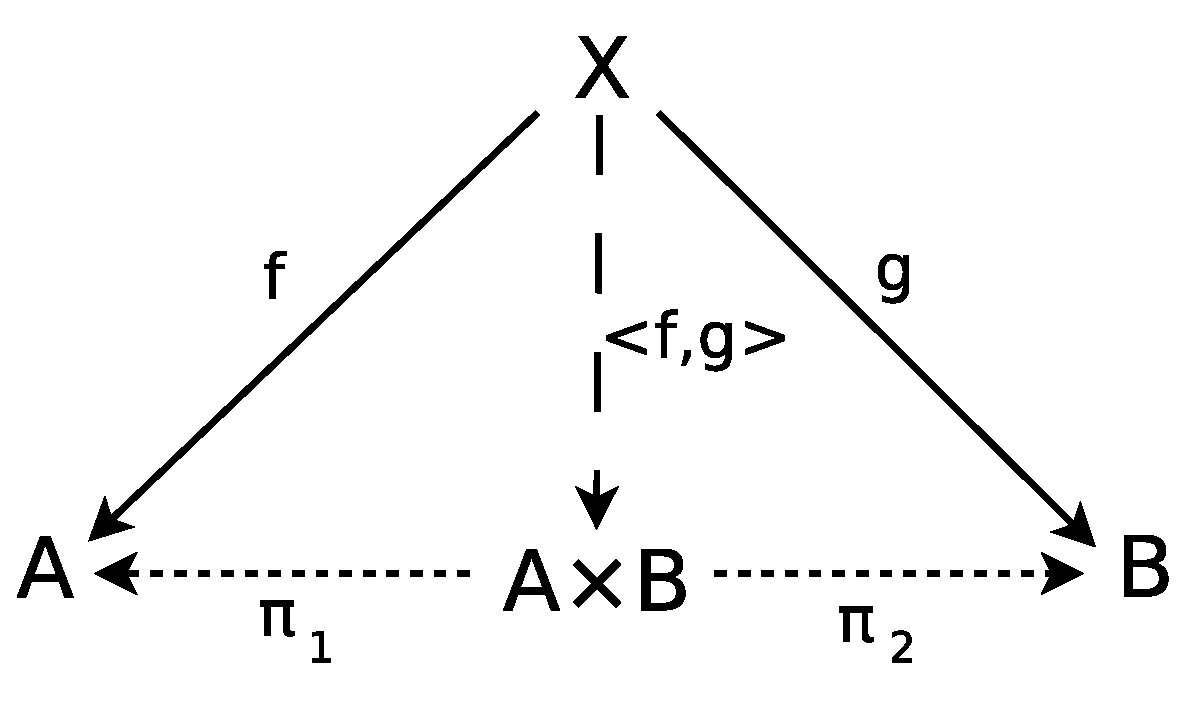
\includegraphics[scale=0.3]{images/cat_product}
    \label{magicl:fig:cat_product}
  }
  \subfloat[Coprodukt]{
    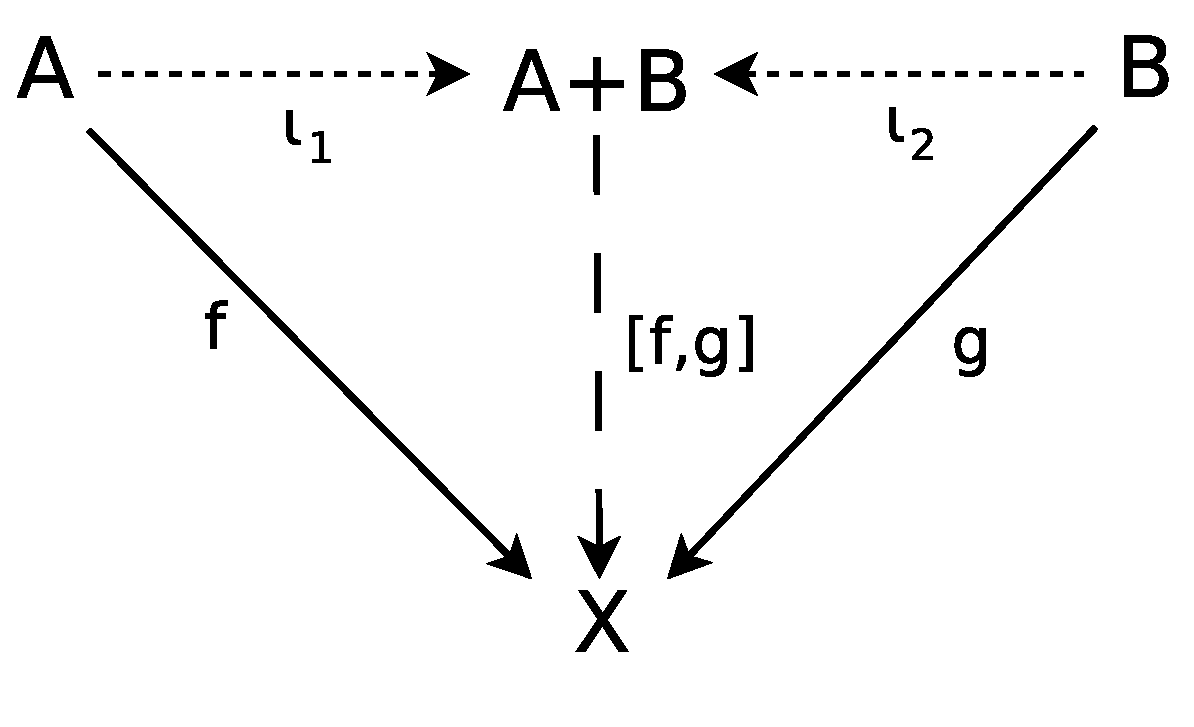
\includegraphics[scale=0.3]{images/cat_coproduct}
    \label{magicl:fig:cat_coproduct}
  }
  \caption{Kommutative Diagramme zur Definition von Produkt und Coprodukt}
\end{figure}

Man kann leicht nachvollziehen, dass das kartesische Produkt genau ein
Produkt für die Kategorie $\mathbf{Set}$ ist. $\langle f,g \rangle$ ist
hier die Funktion, die $x$ auf das Tupel $(f(x), g(x))$ abbildet.

Dreht man im Diagramm alle Pfeile um, erhält man die Definition für das
Coprodukt, einen zum Produkt dualen\footnote{Die zu einer Kategorie
  $\mathbf{C}$ duale Kategorie $\mathbf{C}^{\mathrm{op}}$ entsteht
  nämlich durch das Umdrehen von Pfeilen.} Operator:

\defi{Coprodukt}{ Ein Objekt $A + B$ mit zwei Injektionsmorphismen
  $\iota_1 : A \ato A + B$ und $\iota_2 : B \ato A + B$ ist ein
  Coprodukt von $A$ und $B$, wenn für jedes $X \in \mathrm{Ob}$ sowie
  alle $f : A \ato X$ und alle $g : B \ato X$ genau ein Morphismus
  $[f,g] : A + B \ato X$ existiert, für den \abb{cat_coproduct}
  kommutiert, d.h.  $[f,g] \circ \iota_1 = f$ und $[f,g] \circ \iota_2 =
  g$ gelten.  }

Das Coprodukt entspricht einer disjunkten Vereinigung von Mengen, also
einer Vereinigung von Mengen. die vorher explizit disjunkt gemacht
werden (sofern sie es nicht bereits sind). Dies kann beispielsweise durch
die Indizes $L$ und $R$ geschehen: $\{1,2,3\} + \{2,3,4\} =
\{1_L,2_L,3_L,2_R,3_R,4_R\}$. Der Morphismus $[f,g]$ entspricht einer
Fallunterscheidung: Auf Elemente aus $A$ wird $f$ angewendet, auf welche
aus $B$ entsprechend $g$.

\lsubsection[magicl:cats:func]{Funktoren}

Strukturerhaltende Abbildungen zwischen Objekten und Morphismen zweier
Kategorien werden Funktoren genannt:

\defi{Funktor}{
Ein Funktor $F=(F_{\mathrm{Ob}},F_{\mathrm{Mor}}) : \mathbf{C}
\rightarrow \mathbf{D}$ von Kategorie $C$ nach Kategorie $D$
    \begin{itemize}
    \item bildet jedes Objekt $A \in \mathrm{Ob}^{\mathbf{C}}$ auf $F_{\mathrm{Ob}}(A) \in
      \mathrm{Ob}^{\mathbf{D}}$ ab,
    \item bildet jeden Morphismus $f \in
      \mathrm{Mor}^{\mathbf{C}}_{A,B}$ auf $F_{\mathrm{Mor}}(f) \in
      \mathrm{Mor}^{\mathbf{D}}_{F_{\mathrm{Ob}}(A),F_{\mathrm{Ob}}(B)}$
      ab,
    \end{itemize}
    wobei für alle $A,B,C \in \mathrm{Ob}^{\mathbf{C}}$ und alle $f \in
    \mathrm{Mor^{\mathbf{C}}_{B,C}},g \in
    \mathrm{Mor^{\mathbf{C}}_{A,B}}$ folgende Axiome erfüllt sein
    müssen:
    \begin{itemize}
    \item Erhaltung der Komposition:
      $$F_{\mathrm{Mor}}(f \circ^{\mathbf{C}} g) =
      F_{\mathrm{Mor}}(f) \circ^{\mathbf{D}} F_{\mathrm{Mor}}(g)$$
    \item Erhaltung der Identität:
      $$F_{\mathrm{Mor}}(\mathrm{id}^{\mathbf{C}}_A) =
      \mathrm{id}^{\mathbf{D}}_{F_{\mathrm{Ob}}(A)}$$
    \end{itemize}
}

Statt $F_{\mathrm{Ob}}$ und $F_{\mathrm{Mor}}$ kann einfach $F$
geschrieben werden, wenn aus dem Kontext hervorgeht welche Abbildung
gemeint ist.

Kategorien als Objekte und Funktoren als Morphismen ergeben selbst
wieder eine Kategorie, die Kategorie der kleinen Kategorien - kleine
Kategorien sind Kategorien, deren Klasse von Objekten eine Menge
ist. Diese Einschränkung ist nötig, da Klassen von Klassen in der
Mathematik ähnlich problematisch sind wie Mengen von Mengen.

\lsubsection[magicl:cats:nats]{Natürliche Transformationen}

Eine andere Möglichkeit, aus Funktoren eine Kategorien zu bilden,
besteht darin, diese als Objekte zu benutzen. Alle Funktoren $\mathbf{C}
\ato \mathbf{D}$ als Objekte bilden die sogenannte Funktorkategorie über
$\mathbf{C}$ und $\mathbf{D}$, deren Morphismen natürliche
Transformationen heißen.

\defi{Natürliche Transformation}{Eine natürliche Transformation $\alpha:F \nto
G$ ordnet jedem Objekt $A$ aus $\mathbf{C}$ einen Morphismus
$\alpha_A:F(A) \ato G(A)$ aus $\mathbf{D}$ zu, wobei für alle Objekte
$A,B$ und alle Morphismen $f:A \ato B$ aus $\mathbf{C}$ die
Gleichung
$$\alpha_B \circ F(f) = G(f) \circ \alpha_A $$
gelten muss, was dem kommutativen Diagramm in \abb{cat_nat}
entspricht.
}

Obwohl natürliche Transformationen in der Funktorkategorie Morphismen
sind, werden sie für die bessere Unterscheidung mit $\nto$ statt
$\ato$ notiert.

\fig{cat_nat}{Kommutatives Diagramm in Kategorie $\mathbf{D}$ für die Definition von
  natürlichen Transformationen}

\lsubsection[magicl:cats:monads]{Monaden}

Monaden setzen sich aus einem Endofunktor und zwei natürlichen
Transformationen zusammen:
\defi{Monade}{Eine Monade $(T,\eta,\mu)$ über der Kategorie $\mathbf{C}$ besteht aus
  \begin{itemize}
  \item einem Endofunktor $T:\mathbf{C} \ato \mathbf{C}$,
  \item einer natürlichen Transformation $\eta:\mathrm{id}_{\mathbf{C}} \nto T$,
  \item einer natürlichen Transformation $\mu:T^2 \nto T$,
  \end{itemize}
wobei für jedes Objekt $A$ folgende Axiome erfüllt sein müssen:
\begin{itemize}
\item Assoziativität: $$\mu_A \circ T(\mu_A) = \mu_A \circ \mu_{T(A)}$$
\item Neutrales Element: $$\mu_A \circ T(\eta_A) = \mu_A \circ \eta_{T(A)} = \mathrm{id}_{T(A)}$$
\end{itemize}
}
$\mathrm{id}_\mathbf{C}:\mathbf{C} \ato \mathbf{C}$ bezeichnet hier den Identitätsfunktor,
$\mathrm{id}_{T(A)}:T(A) \ato T(A)$ dagegen den Identitätsmorphismus. Auch diese Gleichungen ließen sich
als kommutative Diagramme darstellen.

Das erste Axiom beschreibt zwei verschiedene Arten, einen Morphismus von
$T(T(T(A)))$ nach $T(A)$ zu bilden: $T(\mu_A):T(T(T(A))) \ato T(T(A))$
auf der linken Seite behält das äußere $T$ bei und verwendet $\mu$, um
das innen stehende $T(T(A))$ in $T(A)$ zu überführen. Rechts reduziert
$\mu_{T(x)}:T(T(T(A))) \ato T(T(A))$ dagegen von außen und lässt das
innere $T(A)$ unangerührt. Wird das Ergebnis dann in $\mu$ gesteckt,
sind innere und äußere Reduktion ununterscheidbar. Die Gleichung lässt
sich auch kurz als $\mu \circ T \mu = \mu \circ \mu T$ schreiben.

Das zweite Axiom funktioniert ähnlich, nur beschreiben diesmal beide
Seiten eine Art, den Identitätsmorphismus für das Objekt $T(A)$ zu
bilden. $T(\eta_A):T(A) \ato T(T(A)$ fügt das neue $T$ innen ein,
$\eta_{T(A)}:T(A) \ato T(T(A))$ hingegen außen.

Zu jeder Monade lässt sich eine neue Kategorie bilden, die Kleisli-Kategorie:
\defi{Kleisli-Kategorie}{
Die Kleisli-Kategorie $\mathbf{C}_K$ zur Kategorie $C$ und der
Monade $(T,\eta,\mu)$ besteht aus
\begin{itemize}
\item den Objekten von $\mathbf{C}$,
\item den Morphismen $f^{\mathbf{C}} \in
  \mathrm{Mor}^{\mathbf{C}}_{A,T(B)}$ aus $C$, die in $f \in
  \mathrm{Mor}^{\mathbf{C}_K}_{A,B}$ umbenannt werden,
\item der Identität $\mathrm{id}_A = \eta_A$,
\item der Komposition $f \circ^{\mathbf{C}_K}_{A,B,C} g = \mu_C
  \circ^{\mathbf{C}} T(f) \circ^{\mathbf{C}} g$.
\end{itemize}
}
Die Erfüllung der Kategorieaxiome wird hier nicht gezeigt, folgt aber
aus den Axiomen für Funktoren, natürliche Transformationen und Monaden.

Monaden sind in der Programmierung nützlich, da sie generisch das
Rechnen mit "`eingepackten"' Werten beschreiben. Beispielsweise könnte
$A$ für den Typ \icode{Int} und $T(A)$ für \icode{List of Int}
stehen. $\eta$ beschreibt dann die Erzeugung einer einelementigen Liste,
$\mu$ reduziert eine Liste von Listen auf eine flache Liste. Über die
Kleisli-Kategorie lassen sich damit bespielsweise nichtdeterministische
Funktionen, die eine Liste möglicher Resultate zurückliefern, elegant
Verknüpfen. Haskell (siehe \sref{haskell}) benutzt Monaden unter
anderem, um Seiteneffekte in eine normalerweise pur funktionale Sprache
einzubauen, wie \sref{magicl:cats_hask:monads} erklärt.

\lsection[magicl:cats_hask]{Kategorien in Haskell}

Die Haskell-Bibliotheken bieten viele kategorientheotische Begriffe an,
die allerdings immer bestimmten Einschränkungen
unterliegen. Beispielsweise sind die Objekte einer Kategorie hier immer
Haskell-Typen. Die Typklasse \icode{Category} ist wie folgt definiert:
\begin{code}
class Category cat where
  id   :: cat a a
  (.)  :: cat b c -> cat a b -> cat a c
\end{code}
Ein Typ \icode{cat}, der selbst zwei Typparameter benötigt, ist also eine
Instanz von \icode{Category}, wenn es generische Identitäts- und
Kompositionsoperatoren gibt, die für beliebige Typen $a,b,c$ benutzt
werden können. Genau genommen bestimmt \icode{Category} also keine
Kategorien, sondern vielmehr die Morphismen bestimmter Kategorien. Auch
die Axiome werden hier nicht gefordert - vielmehr liegt es am
Programmierer, dies für eine "`vernünftige"' Programmsemamtik selbst zu
verifizieren. Man sieht hier schon, dass die Haskell-Begriffe nur sehr
vage mit den mathematischen übereinstimmen - dies wird auch bei den
weiteren Definitionen so bleiben. Die einfachste Instanz von
\icode{Category} ist \icode{(->)}, also die Kategorie der
Haskell-Funktionen, bezeichnet als $\mathbf{Hask}$.
Oft wird statt \icode{.} der \icode{>>>}-Operator (genannt "`vor"') %<<
benutzt mit \icode{f >>> g = g . f}. %<<

\lsubsection[magicl:cats_hask:arrows]{Arrows}

Die Typklasse \icode{Arrow} beschreibt (die Morphismen von) Kategorien,
für die ein Funktor aus der Kategorie $\mathbf{Hask}$ existiert, wo man
also jeder Haskell-Funktion vom Typ \icode{a -> b} einen Morphismus vom
Typ \icode{cat a b} zuordnen kann. Dies ist deshalb sinnvoll, da viele
(Haskell-)Kategorien "`mehr"' können als die Funktionen, formal eine zu
$\mathbf{Hask}$ isomorphe Unterkategorie besitzen. Beispielsweise
benutzt MagicL "`Funktionen, die fehlschlagen können"' oder "`Funktionen
mit Nebeneffekten"' als Kategorien, die jeweils auch normale Funktionen
enthalten. Zusätzlich wird eine Operation auf Tupeln gefordert, aus der
sich ein Produkt zusammensetzen lässt - ein Coprodukt wird zunächst nicht gefordert:
\begin{code}
class (Category ar) => Arrow ar where
  arr   :: (a -> b) -> ar a b
  first :: ar a b  -> ar (a, c) (b, c)
\end{code}
\icode{arr} ist der Funktor, der jede Funktion auf einen Arrow
abbildet\footnote{Die Typen werden hierbei auf sich selbst abgebildet.}.
\icode{first} ist eine Funktion, die aus einem Arrow einen Arrow auf
Tupeln macht, der nur auf dem ersten Element arbeitet, das zweite
dagegen unverändert durchschleift. Somit lassen sich zusätzliche Werte
weiterreichen, außerdem lassen sich aus \icode{first} sinnvolle
Operationen ableiten:

\begin{code}
  second :: ar a b -> ar (c, a) (c, b)
  second = arr swap >>> first f >>> arr swap
    where swap (x, y) = (y, x)

  (***) :: ar a b -> ar a' b' -> ar (a, a') (b, b')
  f *** g = first f >>> second g

  (&&&) :: ar a b -> ar a b' -> ar a (b, b')
  f &&& g = arr diag >>> (f *** g)
    where diag x = (x,x)
\end{code} % <<

\begin{itemize}
\item \icode{second} ist analog zu \icode{first}, reicht allerdings das erste
Element unverändert weiter.
\item \icode{f *** g} wendet \icode{f} auf das
erste Element, danach \icode{g} auf das zweite Element eines Tupels
an.
\item \icode{f &&& g} ist nun die Haskell-Entsprechung von $\langle f,g
\rangle$ in \dref{Produkt}. \icode{f} und \icode{g} werden also beide
auf die Eingabe angewendet und deren Ergebnisse zu einem Tupel
zusammengesetzt.
\end{itemize}

Möchte man einen Arrow mit einer Funktion verknüpfen, gibt es mit
\begin{code}
f >>^ func = f >>> arr func
\end{code}% <<
noch etwas syntaktischen Zucker.

\lsubsection[magic:cats:coproducts]{Coprodukte: Die Klasse \texttt{ArrowChoice}}

Die Haskell-Entsprechung zu einer disjunkten Vereinigung ist der
\icode{Either}-Datentyp, der folgendermaßen definiert ist:
\begin{code}
data Either a b = Left a | Right b
\end{code}
Coprodukte für Arrows werden durch die Klasse \icode{ArrowChoice} beschrieben:
\begin{code}
class (Arrow ar) => ArrowChoice ar where
  left :: ar a b -> ar (Either a c) (Either b c)
\end{code}
Auch hier wird mit \icode{left} nur eine einfache Operation gefordert,
aus der sich anschließend alles weitere konstruieren lässt. Diese
Funktion wandelt einen Arrow von \icode{a} nach \icode{b} um in
einen Arrow von \icode{Either a c} nach \icode{Either b c}. Bei einem
\icode{Left}-Wert wird also der ursprüngliche Arrow angewendet, ein
\icode{Right}-Wert wird dagegen unverändert weitergereicht.
\begin{code}
  right :: ar a b -> ar (Either c a) (Either c b)
  right f = arr swap >>> left f >>> arr swap
    where swap (Left x)  = Right x
          swap (Right x) = Left x

  (+++) :: ar a b -> ar a' b' -> ar (Either a a') (Either b b')
  f +++ g = left f >>> right g

  (|||) :: ar a c -> ar b c -> ar (Either a b) c
  f ||| g = (f +++ g) >>> arr dropEither
    where dropEither (Left x)  = x
          dropEither (Right x) = x

\end{code} %<<
Die Definitionen sind weitgehend analog zu den entsprechenden
Produkt-Operationen:
\begin{itemize}
\item \icode{right} bearbeitet nur \icode{Right}-Werte, während
  \icode{Left}-Werte unverändert bleiben.
\item \icode{f +++ g} wendet auf \icode{Left}-Werte \icode{f} an, auf
  die anderen \icode{g}.
\item Haben \icode{f} und \icode{g} den selben Rückgabetyp, kann
  \icode{f ||| g} verwendet werden, welches das in diesem Fall unnötige
  \icode{Either} verschwinden lässt. Dies entspricht $[f,g]$ in
  \dref{Coprodukt}
\end{itemize}

\lsubsection[magicl:cats_hask:functors]{Funktoren}

Die Haskell-Bibliotheken definieren eine Klasse \icode{Functor}, welche
allerdings nur Endofunktoren über der Kategorie $\mathbf{Hask}$ repräsentieren:
\begin{code}
class Functor f where
  fmap :: (a -> b) -> f a -> f b
\end{code}
Ein Datenkonstruktor \icode{f} ist also Instanz von \icode{Functor},
wenn die Operation \icode{fmap} Funktionen von \icode{a} nach \icode{b}
auf Funktionen von \icode{f a} nach \icode{f b} abbildet. Der
mathematische Funktor besteht hier also aus \icode{(f,fmap)}.

Diese Arbeit benutzt statt dessen eine eigene \icode{Functor}-Klasse,
die Verschiedene Kategorien zulässt:
\begin{code}
class Functor f ar | f -> ar where
  lift :: ar a b -> f a b
\end{code}
Die Arrows \icode{f} und \icode{ar} bilden eine Instanz von
\icode{Functor}, wenn eine \icode{lift}-Operation \icode{ar}-Arrows auf
\icode{f}-Arrows zwischen den gleichen Typen abbildet - wobei der Typ
\icode{f} den Typ \icode{ar} determiniert. Der mathematische Funktor
hier ist also \icode{(id,lift)}. Im Vergleicht zu Haskell's
Standard-\icode{Functor} ist diese Version also in den Kategorien
allgemeiner, aber dafür spezieller in der Abbildung der Objekte, da hier
die Identität vorgeschrieben ist. Man könnte auch dies allgemein
formulieren - aber im Rahmen von MagicL reicht die spezielle Version
bisher aus.

Alle hier verwendeten \icode{Functor}-Instanzen konstruieren aus einem
\icode{Arrow}-Typ einen zweiten mit zusätzlichen Eigenschaften,
z.B. erweitert der \icode{FailFunctor} einen Arrow-Typ um mögliches
Scheitern. Die Instanz-Deklaration dafür sieht im Gerüst folgendermaßen
aus (die Details werden in \sref{magicl:parser:fail} erläutert):
\begin{code}
newtype FailFunctor ar a b = ...

instance (Arrow ar) => Functor (FailFunctor ar) ar where
  lift f = ...
\end{code}

\lsubsection[magicl:cats_hask:monads]{Monaden}

Die Typklasse \icode{Monad} aus den Haskell-Bibliotheken beschreibt
Monaden über der Kategorie $\mathbf{Hask}$. $\eta$ aus
\sref{magicl:cats:monads} heißt hier \icode{return}, statt $\mu$ wird der
Operator \icode{>>=} %<<
mit anderer Signator gefordert:
\begin{code}
class Monad m where
  return :: a -> m a
  (>>=)  :: m a -> (a -> m b) -> m b
\end{code} % <<
Es gibt auch eine genaue Entsprechung von $\mu$, die hier \icode{join}
heißt:
\begin{code}
join :: (Monad m) => m (m a) -> m a
join x = x >>= id
\end{code} % <<

Zu jeder Haskell-Monade \icode{m} lässt sich wieder die
Kleisli-Kategorie bilden, die die Datentypen als Objekte sowie die
Funktionen \icode{a -> m b} als Morphismen enthält. Die
Haskell-Bibliotheken stellen hierfür den Datentyp \icode{Kleisli}
bereit:
\begin{code}
newtype Kleisli m a b = Kleisli (a -> m b)

instance (Monad m) => Category (Kleisli m)
  where id = Kleisli return
        Kleisli f . Kleisli g = Kleisli composed
          where composed x = g x >>= f

instance (Monad m) => Arrow (Kleisli m)
  where arr fun = Kleisli (return . fun)
        first (Kleisli f) = Kleisli tupleF
          where tupleF (x, z) = f x >>= (\ y -> return (y, z))
\end{code} %<<

Arrows und Monaden werden beide verwendet, um abstrakt Verknüpfungen von
speziellen Operationen zu beschreiben. Arrows sind allgemeiner, denn
jede Monade lässt sich beispielsweise mittels \icode{Kleisli} auf einen
entsprechenden Arrow abbilden. Auf der anderen Seite entspricht aber
nicht jedem Arrow eine Monade, denn aus den Arrow-Operationen allein
lässt sich \icode{>>=} % <<
nicht konstruieren. Hierfür wird zusätzlich die Operation \icode{app}
benötigt, die von der Typklasse \icode{ArrowApply} definiert wird (für
Details siehe \cite[S. 18f]{Hughes}):
\begin{code}
class (Arrow ar) => ArrowApply ar where
  app :: ar (ar a b, a) b
\end{code}
Mit \icode{app} wird also ein Arrow bereitgestellt, der als Parameter
einen weiteren Arrow sowie eine Eingabe bekommt, um dann den übergebenen
Arrow auf die Eingabe anzuwenden. Damit ist es möglich, Arrows
einzusetzen, die erst im Verarbeitungsprozess und in Abhängigkeit der
Eingabedaten erzeugt werden - eine Eigenschaft, die Monaden generell
besitzen. Dies wird beispielsweise in \sref{magicl:parser} wichtig für
die Konstruktion von kontextsensitiven Parsern.

Instanzen der Klasse \icode{ArrowChoice} sind vollständig äquivalent zu
Monaden.  Dies wirft die Frage auf, weshalb Haskell überhaupt Monaden
benutzt und nicht alles über Arrows realisiert. Zum einen gibt es dafür
historische Gründe: Monaden waren bereits 1993 in Haskell präsent
\cite[S.23ff]{HaskellHistory}, während Arrows erst 1998 von John Hughes
vorgeschlagen wurden, da sich spezielle Parser mit statischen
Komponenten nicht durch Monaden ausdrücken lassen \cite{Hughes}. Zum
anderen bieten Monaden aber auch Vorzüge: Die Definition einer Monade
ist etwas kürzer, da keine \icode{first}-Funktion für Produkte
bereitgestellt werden muss - wie obiger Code zeigt lässt sich dies
bereits mittels \icode{>>=} % <<
ausdrücken. Zudem gibt es für Monaden in Haskell die praktische
\icode{do}-Notation:
\begin{code}
do x <- foo
   y <- bar x
   return (x, y)
\end{code}
ist syntaktischer Zucker für
\begin{code}
foo >>= (\ x ->
  bar x >>= (\ y ->
    return y))
\end{code} % <<
und ermöglicht eine Schreibweise, die imperativen Programmen ähnelt -
dies ist kein Zufall, da die \icode{IO}-Monade genau für Nebeneffekte
zuständig ist (siehe \sref{magicl:cats_hask:monads:examples:io}). Diese
Verwendung erklärt auch nachträglich den Namen \icode{return}, wobei es
sich noch immer um die $\eta$-Transformation handelt und nicht etwa ein
syntaktisches \icode{return}-Statement wie in imperativen Sprachen
üblich.

Für Arrows gibt es mit \icode{proc} auch eine Notation, mit der
Zwischenergebnisse benannt werden können. Diese ist aber weniger simpel
und elegant als das Monadenäquivalent. Auf der anderen Seite eignen sich
Arrows besser als Monaden für eine punktfreie Schreibweise, d.h. einer
Schreibweise ohne Zwischenvariablen, bei der ausschließlich auf
Komposition zurückgegriffen wird. Punktfreie Notation wird auch bei
Definitionen von Funktionen oft verwendet und ist für viele
Haskell-Programmierer natürlicher und eleganter.

\lsubsubsection[magicl:cats_hask:monads:examples]{Beispiele für Monaden}

\lparagraph[magicl:cats_hask:monads:examples:maybe]{\icode{Maybe}}

Funktionen, die fehlschlagen können, lassen sich in der Form \icode{a
  -> Maybe b} darstellen. Möchte man mehrerer solcher Funktionen
verketten, werden normalerweise viele Fallunterscheidungen benötigt, da
bei jeder Funktion die Rückgabe geprüft und nur im Erfolgsfall die
nächste aufgerufen muss. Haskell vereinfacht dies, indem \icode{Maybe}
zur Monade erklärt wird:
\begin{code}
instance Monad Maybe
  where return = Just
        (Nothing >>= _) = Nothing
        (Just x  >>= f) = f x
\end{code} % <<
Obiges Codebeispiel
\begin{code}
do x <- foo
   y <- bar x
   return (x, y)
\end{code}
würde in der Maybe-Monade so interpretiert werden: Wenn \icode{foo}
erfolgreich ist, wird das Ergebnis (lokal) in \icode{x} gespeichert. Ist
daraufhin \icode{bar x} ebenfalls erfolgreich, wird dieses in \icode{y}
gespeichert und als Ergebnis \icode{Just (x, y)} zurückgegeben. Schlägt
eine der Funktionen fehl, ist das ergebnis \icode{Nothing}.

\lparagraph[magicl:cats_hask:monads:examples:io]{\icode{IO}}

Jede Programmiersprache benötigt für die reale Welt Möglichkeiten,
Operationen mit Nebeneffekten wie das Schreiben oder solche, die von
externen Nebeneffekten abhängen, wie das Lesen von Dateien,
auszuführen. Dies lässt sich zunächst schwer in eine puren Sprache wie
Haskell integrieren. Die \icode{IO}-Monade bietet hier eine Lösung: Man
stelle sich einen fiktiven Datentyp \icode{World} vor, der den gesamten
Zustand der externen Welt enthält. \icode{IO a} ist nun eine Funktion,
die die Welt liest und eine andere Welt sowie ein a zurückgibt:
\begin{code}
newtype IO a = World -> (World, a)
\end{code}
Zum Verketten zweier \icode{IO}-Operationen wird die von der ersten
zurückgegebene Welt an die zweite übergeben. Damit dies nicht von Hand
geschehen muss, wird \icode{IO} wieder als Monade deklariert. Nun gibt
es aber natürlich keinen wirklichen \icode{World}-Typen - in
Wirklichkeit wird also der Haskell-Compiler alles, was mit \icode{IO}
verpackt ist, in imperativen Code übersetzen. Dennoch gelingt dadurch
die saubere Trennung von puren Code und solchem, der Nebeneffekte
enthalten kann. Da ist nicht möglich ist, eine "`Auspack-Funktion"'
\icode{IO a -> a} zu definieren\footnote{Es gibt eine solche Funktion in
  Haskell, die aber normalerweise nicht verwendet werden sollte.}, das
Gegenteil aber mit \icode{return} möglich ist, kann imperativer Code
immer funktionalen, funktionaler Code aber niemals imperativen
enthalten. Die äußerste Funktion jedes Haskell-Programms, \icode{main},
wird deshalb immer in der \icode{IO}-Monade ausgeführt.

Dank der Kleisli-Kategorie lassen sich mittels \icode{IO} auch Arrows
bereitstellen, die Nebeneffekte enthalten:
\begin{code}
type IOArrow = Kleisli IO
\end{code}

\lsection[magicl:parser]{Parser als Arrows}

Das Herzstück von MagicL ist ein Arrow-basiertes Framework für die
Konstruktion von Parsern. Die obersten Ziele sind Allgemeinheit sowie
sinnvolle Ausgaben im Fehlerfall. Mit Allgemeinheit sind zwei
Anforderungen gemeint: Zum einen sollen beliebige Streams gelesen
werden können und nicht etwa nur Zeichenketten, damit auch \sexps{}
verarbeitet werden können und so eine Art alternativer Makroprozessor
erstellt wird. Zum anderen soll das Interface so allgemein sein, dass
später beliebige andere Parser-Architekturen integriert werden können.

Haskell besitzt mit Parsec\cite{Parsec} bereits eine sehr
performante und praktische Parser-Kombinator-Bibliothek, die auf Monaden
basiert. Diese ist allerdings auf die Verarbeitung von Zeichenketten
beschränkt, weshalb sie in MagicL keine Verwendung findet.

MagicL benutzt Arrows und Funktoren, um möglichst allgemein zu
sein. Alles, was im Rahmen dieser Arbeit implementiert wurde, hätte zwar
auch über Monaden und Monaden-Transformatoren konstruiert werden
können. Dennoch besteht die Möglichkeit, dass später Ergänzungen
vorgenommen werden sollen, die sich nicht mittels Monaden ausdrücken
lassen - beispielsweise ein effizienterer Parsing-Algorithmus, der
sowohl statische als auch dynamische Komponenten enthält, wie ihn
Swierstra und Duponcheel entworfen haben (siehe \cite[S. 8ff]{Hughes}).

Wenn, wie in Parsec möglich (siehe \cite[S. 3]{Parsec}),
kontextsensitive Parser - beispielsweise für die Zuordnung von
schließenden Tags in XML-Dokumenten - konstruiert werden sollen,
müssen die zugrundeliegenden Arrows allerdings äquivalent zu Monaden
sein und \icode{ArrowApply} implementieren

Dieser Abschnitt entwickelt nun schrittweise einen Parser-Datentyp aus
Arrows. Parser zeichnen sich hauptsächlich durch zwei Eigenschaften aus:
\begin{itemize}
\item Sie können fehlschlagen sowie Alternativmöglichkeiten im Falle des
  Scheiterns besitzen.
\item Sie bearbeiten einen Zustand, der die Position im Eingabestream
  beschreibt.
\end{itemize}
Diese beiden Eigenschaften lassen sich einzeln mittels Funktoren auf
bestehenden Kategorien ausdrücken.

\lsubsection[magicl:parser:fail]{Fehlschlagende Arrows}

Berechnungen von $A$ nach $B$, die fehlschlagen können, sollen zwei
mögliche Resultate haben. Im Erfolgsfall wird ein normaler Rückgabewert
aus $B$ geliefert, während im Falle eines Scheiterns eine Fehlermeldung
als String zurückgegeben wird - im Gegensatz zur \icode{Maybe}-Monade,
die im Fehlerfall nur ein \icode{Nothing} liefert. Der Rückgabetyp ist
deshalb das Coprodukt $\mathrm{String}+B$. Statt Morphismen von $A$ nach
$B$ wollen wir also nun Morphismen von $A$ nach $\mathrm{String}+B$. Um
den aufrufenden Code nicht komplizierter zu machen, empfiehlt es sich,
diese Änderung in einer neuen Kategorie $\mathbf{C}_f$ zu
verstecken. $f_{f} : A \rightarrow B$ aus der neuen Kategorie wird
abgebildet auf $f : A \rightarrow \mathrm{String} + B$ Der Arrow
$\mathrm{fail}_{f} : \mathrm{String} \rightarrow a$ in $C_{f}$ schlägt
immer fehl und entspricht $fail : \mathrm{String} \rightarrow
\mathrm{String} + a$ in $C$.

Der Operator $\bigvee : Mor_{A,B} \times Mor_{A,B}
\rightarrow Mor_{A,B} $ bietet Alternativen. Um Morphismen aus
$\mathbf{C}$ in $\mathbf{C}_f$ benutzen zu können, gibt es den Funktor
$\mathrm{lift}_f:\mathbf{C} \ato \mathbf{C}_f$, welcher die
unveränderte, d.h. gelingende Operation für die neue Kategorie
übernimmt.

Die Haskell-Entsprechung von $\mathrm{String}+B$ ist \icode{Either
  String b}, was sich mit \icode{Failable b} abkürzen lässt, wenn man
den parametrisierten Typ \icode{Failable} einführt:

\begin{code}
type Failable a = Either String a
\end{code}

Der Fehlerfall wird durch \icode{Left String} ausgedrückt, ein Erfolg
durch \icode{Right a}. Fehlschlagende Arrows nun sind in MagicL durch den
Typ \icode{FailFunctor} implementiert:

\begin{code}
newtype FailFunctor ar a b = FailF (ar a (Failable b))

instance (Arrow ar) => Functor (FailFunctor ar) ar where
    lift f = FailF (f >>> arr Right)
\end{code} % <<

Arrows von \icode{a} nach \icode{b}, die fehlschlagen können, sind also
Arrows von \icode{a} nach \icode{Failable b}, die in den zusätzlichen
Konstruktor \icode{FailF} eingebettet wurden. Um einen normalen Arrow
\icode{f} aus \icode{ar} nach \icode{FailFunctor ar} zu "`liften"', wird
der Rückgabewert in ein \icode{Right} gebettet und der resultierende
Arrow in \icode{FailF}.
Der Arrow \icode{fail} wird in eine \icode{Arrow} erweiternde Typklasse
ausgegliedert, so dass dieser auch in anderen Kategorien bereitgestellt
werden könnte:

\begin{code}
class (Arrow ar) => ArrowFail ar where
  fail :: ar String a

instance (ArrowChoice ar) => ArrowFail (FailFunctor ar) where
  fail = FailF (arr Left)
\end{code}

Der Oder-Operator $\bigvee$ entspricht in Haskell \icode{<+>}, welchen
die bereits in den Haskell-Bibliotheken definierte Typklasse
\icode{ArrowPlus} bereitstellt:

\begin{code}
instance (ArrowChoice ar) => ArrowPlus (FailFunctor ar) where
  FailF f <+> FailF g = FailF ((f &&& g) >>> arr tupleOr)
    where tupleOr (Left  _, y)  = y
          tupleOr (Right x), _) = Right x
\end{code} % <<

Es werden also \icode{f} und \icode{g} parallel evaluiert und
anschließend von der Funktion \icode{tupleOr} verarbeitet, die, sollte
\icode{f} fehlschlagen, das Ergebnis von \icode{g} zurückgibt, ansonsten
das Ergebnis von \icode{f}.

\fig{cat_fail}{Komposition beim Fail-Funktor}

Die Typabhängigkeit von \icode{ArrowChoice} ist nötig, weil
\icode{FailFunctor ar} nur dann ein \icode{Arrow} ist, wenn \icode{ar}
ein Coprodukt anbietet. Denn die Komposition in $C_{f}$ ist definiert
durch $g_{f} \circ f_{f} = ([fail,g] \circ f)_{f}$, was in Haskell
\begin{code}
FailF g . FailF f = FailF (f >>> (arr Left ||| g))
\end{code} %<<
entspricht. Tritt in \icode{f} ein Fehler auf, wird dieser also wieder
in ein \icode{Left} eingepackt und zurückgegeben. Ansonsten wird das
durch \icode{|||} implizit aus dem \icode{Right}-Konstruktor ausgepackte
Ergebnis an \icode{g} weitergereicht.

\abb{cat_fail} zeigt die Komposition in $\mathbf{C}_f$ und deren
zurückführung auf ein Coprodukt in $\mathbf{C}$. Die Funktion, die $f_f$
auf $f$ abbildet, kann nicht Teil eines Funktors sein. Ein solcher
müsste nämlich das Objekt $B$ sowohl auf $\mathrm{String}+B$ (bei der
Transformation von $f$ als auch auf $B$ selbst (bei $g$) abbilden.

\todo{(Co)Produkt?}

\lsubsection[magicl:parser:state]{Arrows mit Zuständen}

Zustände lassen sich ähnlich zu einem Arrow hinzufügen. Über Produkte
wird der Zustandstyp $S$ (z.B. eine Stream-Position oder der
\textit{Seed} eines Zufallszahlengenerators) an Domäne und Codomäne
herangehängt, was wieder in einer neuen Kategorie $C_{s}$ versteckt
wird. Ein Morphismus $f_{s} : A \rightarrow B$ der neuen Kategorie wird
entsprechend abgebildet auf $f = A \times S \rightarrow B \times S$. Da
hier im Gegensatz zum Fail-Funktor Domäne und Codomäne gleich abgebildet
werden, ist diese Abbildung Teil eines Funktors $F_s: C_{s}
\ato C$. \abb{cat_state} zeigt d

\fig{cat_state}{Komposition in $\mathbf{C}_s$ und Rückführung auf
  $\mathbf{C}$ durch $F_s$}

In MagicL gibt es die Typklasse \icode{StateFunctor}, die einen weiteren
Typparameter \icode{s} für den Zustand bekommt:

\begin{code}
newtype StateFunctor s ar a b = StateF (ar (a, s) (b, s))

instance (Arrow ar) => Functor (StateFunctor s ar) ar where
    lift = StateF . first
\end{code} % <<

Die "`geliftete"' Version eines Arrows soll den Zustandsparameter
unverändert weitergeben - dies entspricht genau der
\icode{first}-Funktion aus \sref{magicl:cats_hask:arrows}.

Das Lesen und Schreiben von Zuständen wird von den Funktionen \icode{get} und
\icode{put} bereitgestellt, welche in der Typklasse \icode{ArrowState}
definiert werden:

\begin{code}
class (Arrow ar) => ArrowState s ar | ar -> s where
  get :: ar a s
  put :: ar s ()

instance (Arrow ar) => ArrowState s (StateFunctor s ar)
  where
    get = StateF (arr (\ (_, state) -> (state, state)))
    put = StateF (arr (\ (state, _) -> ((), state)))
\end{code}

\icode{get} ignoriert also den Eingabewert und gibt den aktuellen
Zustand zurück, während \icode{put} den übergebenen Zustand
"`abspeichert"' und (bis auf diesen) nichts zurückgibt.

\todo{Prod/Coprod?}

\lsubsection[magicl:parser:parse]{Der Parse-Funktor}

Nun lassen sich obige Kategorie-Erweiterungen zu einer Parser-Kategorie
$\mathbf{C}_p = \mathbf{C}_{fs}$ zusammensetzen, d.h. die ursprüngliche
Kategorie wird zunächst um Fehler zu $\mathbf{C}_f$, danach um Zustände
zu $\mathbf{C}_p$ erweitert. Die Reihenfolge hier ist wichtig, damit ein
Morphismus $A \ato B$ aus $\mathbf{C}_p$ auf $A \times S \ato
\mathrm{String} + B \times S$ in $\mathbf{C}$ abgebildet wird und nicht
auf $A \times S \ato (\mathrm{String} + B) \times S$, wie es andersherum
wäre. Denn das Coprodukt muss "`außen"' stehen, um im Kontrollfluß
zuerst bearbeitet zu werden und somit ein Backtracking im Fehlerfall zu
ermöglichen.

Backtracking wird allerdings zu einem Problem, wenn man sinnvolle
Fehlermeldungen produzieren will. Man stelle sich einen Parser für die
(in einer fiktiven Sprache beschriebene) Grammatik \texttt{\{.*\}
  $\bigvee$ [.*]} vor, die eine beliebige Zeichenkette in geschweiften
oder eckigen Klammern beschreibt. Beim Eingabewort \texttt{\{ABC}
scheitert zunächst aufgrund der fehlenden schließenden Klammer die erste
Alternative, woraufhin die zweite probiert wird. Das Wort beginnt aber
nicht mit \texttt{[}, so dass der Parser beispielsweise mit der Meldung
\texttt{"'Expected [, got \{"'} scheitert. Diese Meldung beschreibt den
Fehler schlecht - statt dessen möchte man nach dem Lesen von \texttt{\{}
das Backtracking deaktivieren, denn bereits hier ist klar, dass die
andere Alternative nicht mehr in Betracht kommt. Dies führt zu einer
sinnvolleren Fehlermeldung wie \texttt{"'Expected \}, got end of
  stream"'}.

Ein derartiger "`nicht-auffangbarer"' Fehler lässt sich durch das
Einbauen einer weiteren Möglichkeit des Scheiterns ermöglichen, wir
definieren also $\mathbf{C}_p = \mathbf{C}_{ffs}$ und bieten eine
Funktion \icode{forceParser} an, die einen (Sub-)Parser derart
modifiziert, dass, falls dieser Scheitert, der Fehler in die "`inneren"'
und damit nicht-recover-fähigen Fail-Kategorie übernommen wird. Hiervon
wird beispielsweise bei der Funktion \icode{macro}
\sees{magicl:sexp} Gebrauch gemacht.

Die Haskell-Definition vom \icode{FailFunctor} benutzt als Zustandstyp
einen Stream (als Liste repräsentiert) vom Token-Typ \icode{t}:

\begin{code}
newtype ParseFunctor t ar a b =
  P (StateFunctor
     [t]
     (FailFunctor (FailFunctor ar))
     a
     b)
\end{code}

Dank der Implementation als Funktor ist die Kategorie, in der der Parser
ausgeführt wird, frei wählbar. So können rein funktionale Parser in
$Hask_p$ konstruiert werden. Benötigt man aber Debug Outputs (z.B. bei
der Suche einer Endlosschleife) oder andere Seiteneffekte, kann
$\mathbf{IO}_p$ benutzt werden. In MagicL werden diese Kategorien durch
die Typaliase \icode{FunParser} wowie \icode{IOParser} bereitgestellt:
\begin{code}
type FunParser t a b = ParseFunctor t (->) a b
type IOParser  t a b = ParseFunctor t IOArrow a b
\end{code}
Eine geeignete innere Kategorie könnte
sogar interaktive Debugger, Netzwerktransparenz oder sonstige Features
anbieten. Auch der variable Token-Typ erzeugt viele Möglichkeiten:
Textdateien können mit \icode{Char}, Bitstreams mit \icode{Bool} oder
\sexp{}-Streams mit \icode{Sexp} verarbeitet werden.

\lsubsection[magicl:parser:lib]{Parser-Library}

MagicL beinhaltet eine Parser-Bibliothek, in der u.a. viele simple
Parser-Konstruktoren definiert sind. Hier ein paar
Beipiele\footnote{Abhängigkeiten der Typparameter werden hier der
  Übersichtlichkeit halber weggelassen.}:
\begin{itemize}
\item \icode{empty :: ParseFunctor t ar a a}\\
  gibt seinen Eingabewert unverändert zurueck, wenn der Stream leer ist.
\item \icode{takeWhen :: (t -> Bool) -> (t -> String) -> ParseFunctor t ar a
    t}\\
  testet den ersten Token mit einem Prädikat. Im Erfolgsfall (\icode{True}) wird der
  Token zurückgegeben, ansonsten wird der Token an eine Funktion
  übergeben, die daraus eine Fehlermeldung aufbaut.
\item \icode{member :: [t] -> ParseFunctor t ar a t}\\
  testet, ob der erste Token in der übergebenen Liste vorkommt.
\item \icode{streamEq ::  [t] -> ParseFunctor t ar a [t]}\\
  prüft, ob die ersten $n$ Token mit den Elementen der übergebenen Liste
  übereinstimmen, und gibt diese im Erfolgsfall zurück. Für \icode{t =
    Char} wird hier also ein String gelesen.
\end{itemize}

Alle diese Funktionen (und deren Negationen) geben Parser mit nützlichen
Fehlermeldungen zurück.

Weiterhin gibt es viele Arrow-Kombinatoren, mit denen Parser,
vergleichbar mit den Operationen der Erweiterten Backus-Naur-Form (EBNF)
\cite{TODO}, verschaltet werden können. Mit den bisher eingeführten
Operatoren sind bereits Konkatenation (\icode{>>>}) %<<
und Alternative (\icode{<+>}) abgedeckt, darüber hinaus gibt es für
Instanzen von \icode{ArrowPlus} unter anderem folgende Funktionen:

\begin{code}
optional :: (...) => ar a b -> ar a (Maybe b)
optional f = (f >>^ Just) <+> constArrow Nothing
  where constArrow x = arr (\ _ -> x)

many :: (...) => ar a b -> ar a [b]
many f = many1 f <+> constArrow []

many1 :: (...) => ar a b -> ar a [b]
many1 f = consArrow f (many f)
  where consArrow :: ar a b -> ar a [b] -> ar a [b]
        consArrow f g = (f &&& g) >>^ (\ (x,xs) -> x : xs)

skip :: (...) => ar a b -> ar a a
skip f = (f &&& id) >>^ snd

sepBy :: (...) => ar a c -> ar a b -> ar a [b]
sepBy sep item =
  optional (consArrow item (many (skip sep >>> item))) >>^ unMaybeList
    where
      unMaybeList  Nothing  = []
      unMaybeList (Just xs) = xs
\end{code} % <<

\icode{optional} erzeugt einen Arrow, der, sollte der übergebene Arrow
scheitern, \icode{Nothing} zurückgibt - dabei aber "`erfolgreich"'
bleibt. Dies entspricht \icode{[ ]} in EBNF. Hierbei erzeugt
\icode{constArrow Nothing} einen Arrow, der die Eingabe ignoriert und
konstant \icode{Nothing} zurückgibt. Eine (optionale) Wiederholung (in EBNF
\icode{\{ \}}) erzeugt \icode{many}, \icode{many1} verlangt mindestens
ein Vorkommen. Die Hilfsfunktion \icode{consArrow} nimmt zwei
Arrows an und erzeugt daraus einen, der das Element, welches der erste
zurückgibt, vor die Liste hängt, die der zweite zurückliefert.
\icode{skip} ignoriert das Resultat eines Arrows und gibt
statt dessen seine Eingabe zurück - Zustandsänderungen kann der
ignorierte Arrow aber dennoch bewirken. \icode{sepBy} ist ein
komplizierteres Beispiel und ermöglicht das Parsen von Listen mit
Trennzeichen. Dafür bekommt die Funktion zwei Arrows übergeben:
\icode{sep} soll ein Trennzeichen, \icode{item} ein Element lesen. Es
wird zunächst ein \icode{item}, dann beliebig viele, von (ignorierten)
\icode{sep} angeführte \icode{item}-Elemente gelesen. Das ganze ist noch
in ein \icode{optional} gebettet, damit auch eine leere Liste gelesen
werden kann. Die Rückgabe wird mittels \icode{unMaybeList} vom durch
\icode{optional} erzeugten \icode{Maybe}-Datentyp befreit, so dass statt
\icode{Nothing} eine leere Liste zurückgegeben wird, wenn nichts gelesen
werden kann.

\lsubsubsection[magicl:parser:lib:example]{Beispiel: Ein \sexp{}-Parser}

Aufgrund der einfachen gewählten Struktur von \sexps{} und der
praktischen Parser-Library ist es möglich, in vier kurzen Zeilen einen
Parser für \sexps{}\footnote{Gemeint ist ein Parser von Text nach
  \sexps{}, wogegen die \sexp{}-Parser in \sref{magicl:sexp} \sexps{}
  lesen.} zu entwerfen:

\begin{code}
whitespace = skip (many (member " \t\n"))
\end{code}
Zunächst wird Whitespace als beliebige Anhäufung von Spaces, Tabs und
Newlines definiert, die ignoriert werden soll.
\begin{code}
parseSymbol = many1 (notMember " \t\n()") >>^ Symbol
\end{code} % <<
Ein Symbol ist eine Kette von Zeichen, die weder Whitespace noch
Klammern sind. Dieses wird gleich an den \icode{Symbol}-Konstruktor
übergeben, um den Typ \icode{Sexp} zu erhalten.
\begin{code}
parseNode = skip (eq '(') >>> (many parseSexp >>^ Node) >>> skip (eq ')')
\end{code} % <<
Ein Knoten ist eine von Klammern umgebene Liste von \sexps{}, die
mittels \icode{Node}-Konstruktor zu einem \sexp{} wird.
\begin{code}
parseSexp = whitespace >>> (parseSymbol <+> parseNode) >>> whitespace
\end{code} % <<
Ein \sexp{} ist nun entweder ein Symbol oder ein Knoten, wobei davor und
danach Whitespace auftreten darf.

Tritt bei Lesen ein Fehler auf, wird automatisch eine brauchbare Fehlermeldung
ausgegeben, z.B.

\begin{code}
"(test) )"  ==>  Empty stream expected: ")"
\end{code}

\lsection[magicl:sexp]{Parsen von \sexps{}}

\todo{SexpParser Typ}

Die Parser-Bibliothek an sich ist bereits nützlich, um Textdateien
einlesen zu können. Das eigentliche Ziel aber ist die Verarbeitung von
\sexps{}. Es lassen sich zwar bereits Streams von \sexps{} verarbeiten,
es gibt aber bisher keine komfortablen Operationen, um das Innere einer
\sexp{} zu testen oder zu verarbeiten. Da ein \sexp{} selbst wieder eine
Liste und damit ein Stream ist, bietet es sich an, diesen ebenfalls über
einen "`inneren Parser"' zu verarbeiten.

Beispielsweise könnte eine Liste von Personen folgenderweise
repräsentiert sein\footnote{Dieses Format ist unnötig redundant und
  sollte vermutlich besser durch \icode{(persons Franz Walter Heinz)} ersetzt
  werden - aber es handelt sich ja nur um ein einfaches Beispiel.}:
\begin{code}
(person Franz)
(person Walter)
(person Heinz)
\end{code}

Ein Parser, der eine Liste von Namensstrings produzieren soll, würde mit
der bisherigen Bibliothek so aussehen:

\begin{code}
parsePerson :: SexpParser String
parsePerson = take >>^ proc >>> (fail ||| id)
  where proc (Node [Symbol "person", Symbol x]) = Right x
        proc _ = Left ("Not a person: " ++ show x)
parsePersons :: SexpParser [String]
parsePersons = many parsePerson
\end{code} % <<

Die Verarbeitung von Hand mittels \icode{Node} und \icode{Symbol} im
Pattern-Matching ist relativ umständlich. Deswegen gibt es eine Reihe
nützlicher Hilfsfunktionen für die Konstruktion von \sexp{}-Parsern:

\begin{itemize}
\item \icode{takeSexp} liest eine \sexp{} vom Stream und wandelt diese
  für die Unterscheidung zwischen Symbolen und Knoten mittels
  \icode{|||} in das Coprodukt \icode{Either String [Sexp]} um.
\item \icode{takeSymbol} erwartet ein Symbol und gibt dieses als String
  zurück - ansonsten wird eine Fehlermeldung ausgegeben.
\item \icode{symbolMacro name = skip (eq (Symbol name))} akzeptiert nur
  das Symbol mit Namen \icode{name}.
\item \icode{takeNode} erwartet einen Knoten und gibt diesen als Liste
  von \sexps{} zurück.
\item \icode{compNode innerComp} verarbeitet einen Knoten, indem der
  übergebene Parser \icode{innerComp} auf das Knoteninnere angewendet
  wird. Da Parser in MagicL immer als Compiler definiert werden (siehe
  \sref{magicl:arch:compiler}), heißt diese Funktion nicht \icode{parseNode}
\item \icode{macro name innerComp} % <<
  konsturiert nun einen Parser, der wie ein Macro das erste Element des
  Knotens mit dem Symbol \icode{name} vergleicht und im Erfolgsfall die
  restlichen Elemente mit \icode{innerComp} verarbeitet. Danach wird
  sichergestellt, dass der Knoten auch wirklich vollständig gelesen
  wurde - will man dies nicht, da man den Rest ignoriert, gibt es die
  Funktion \icode{looseMacro} mit identischer Signatur.
\end{itemize}
Das obige Beispiel lässt sich nun umschreiben:
\begin{code}
parsePerson  = macro "person" takeSymbol
parsePersons = many parsePerson
\end{code}

\icode{macro} benutzt \icode{forceParser} aus
\sref{magicl:parser:parse}, um das Backtracking auszuhebeln, sobald das
Symbol übereinstimmt, was wieder für bessere Fehlermeldungen
sorgt. Allerdings bedeutet dies, dass Code wie
\begin{code}
macro "foo" (symbolMacro "bar") <+> macro "foo" (symbolMacro "baz")
\end{code}
nicht erwartungsgemäß funktioniert:
\begin{code}
(foo bar)   => ()  d.h. Erfolg, kein Ergebnis
(foo baz)   => Symbol bar expected: baz
\end{code}
Es sollte deshalb immer nur ein \icode{macro} für jeden Begriff benutzt
werden, und eine Oder-Verknüpfung ins Innere verlegt werden - hier also:
\begin{code}
macro "foo" (symbolMacro "bar" <+> symbolMacro "baz")
\end{code}

\lsection[magicl:arch]{Rahmenarchitektur}

Um das Parser-Framework herum soll ein wieder möglichst allgemeines
Interface für die beschreibung von Compilern bestehen. Ziel ist die
selbstständige Suche nach einem passenden Compiler, wenn nur Ein- und
Ausgabetyp spezifiziert sind. Compiler sollen unter anderem als pure
Funktionen oder als Parser spezifiziert werden können.

Ein Compiler von \icode{a} nach \icode{b} ist in MagicL etwas, was sich
in eine Operation mit \icode{a} als Ein- und \icode{b} als Ausgabe
überführen lässt. Diese Operation kann im allgemeinen Nebeneffekte
enthalten, weshalb IOArrow verwendet wird. Typen, mit denen sich
Compiler repräsentieren lassen, implementieren die Typklasse
\icode{Executable}:
\begin{code}
class Executable x a b | x -> a b where
  toIO :: x -> IOArrow a b
\end{code}
\icode{x} ist selbst ein parametrisierter Typ, der die Ein- und
Ausgabetypen \icode{a} und \icode{b} bereits determiniert. Die einfachsten
Instanzen von \icode{Executable} werden durch IOArrows selbst sowie pure
Funktionen gebildet:
\begin{code}
instance Executable (IOArrow a b) a b where
  toIO = id

instance Executable (a -> b) a b where
  toIO f = Kleisli (return . f)
\end{code}
Auch Parser sind ausführbar, sofern der zugrundeliegende Arrow-Typ es
ist:
\begin{code}
instance (...) => Executable (ParseFunctor t ar () a) [t] a where
  toIO = toIO . execParser
\end{code}

Nun soll es möglich sein, einen ausführbaren Typen zu benutzen, um einen
eindeutigen Compiler von \icode{a} nach {b} einzurichten. Dies geschieht
über die Typklasse \icode{Compilable}:
\begin{code}
class (Executable x a b) => Compilable x a b | a b -> x where
  comp :: x
\end{code}
Da es nur einen ausgezeichneten Compiler von \icode{a} nach \icode{b}
geben kann, determinieren \icode{a} und \icode{b} gemeinsam \icode{x},
wobei die umgekehrte Abhängigkeit ebenfalls - von \icode{Executable}
geerbt - besteht. Es handelt sich also um eine 1:1-Beziehung. Die
spezifikation eines simplen funktionalen Compilers würde so aussehen:
\begin{code}
instance Compilable (A -> B) A B where
  comp x = ...
\end{code}
Der Parser, der Strings in Listen von \sexp{} einliest, wird auch als
Compiler spezifiziert:
\begin{code}
instance Compilable (FunParser Char () [Sexp]) String [Sexp] where
  comp = many parseSexp
\end{code}
Die Typklasse \icode{Compiler} "`vergisst"' nun den zur Definition
verwendeten Typen:
\begin{code}
class Compiler a b where
  compile :: IOArrow a b

instance (Compilable x a b) => Compiler a b where
  compile = toIO comp
\end{code}
Nun kann ein beliebiger Compiler einfach über einen explizit typisierten
\icode{compile}-Aufruf, wie etwa \icode{compile :: IOArrow String
  [Sexp]}, gefunden

MagicL enthält zudem ein minimalistisches Testframework, um Compiler
oder im speziellen Macros inkrementell zu testen.

\lsection[magicl:code]{\cgen{}}

Um komfortabel korrekt eingerückten Code in einer Zielsprache generieren
zu können, stellt MagicL einen Datentyp \icode{Code} zur Verfügung,
sowie einen Compiler von \icode{Code} nach \icode{String}, welcher ein
Nachbau des von Philip Wadler in \cite[S.223ff]{FunOfProgramming}
vorgestellten Pretty-Printers ist. Die elementaren
Konstruktor-Funktionen sind:
\begin{code}
newline :: Code
text    :: String -> Code
append  :: Code   -> Code -> Code
group   :: Code   -> Code
indent  :: Int    -> Code -> Code
\end{code}

\icode{newline}, \icode{text} und \icode{append} sollten selbsterklärend
sein. \icode{group} versucht den übergebenen \icode{Code} auf eine Zeile
zu bekommen, indem es alle Zeilenumbrüche durch Leerzeichen
ersetzt. Wird dabei allerdings die geforderte Zeilenlänge (im
Standard-Compiler 70) überschritten, wird die ursprüngliche Version mit
Zeilenumbrüchen genommen. \icode{indent} rückt den übergebenen
\icode{Code} bei jedem Zeilenumbruch um $n$ Zeichen ein, z.B. würde
\begin{code}
indent 2 (conc [text "hallo", newline, text "welt"])
\end{code}
den Text
\begin{code}
hallo
  welt
\end{code}
ergeben - dabei verbindet \icode{conc :: [Code] -> Code} eine Liste
mittels \icode{append}. Darüber hinaus gibt es viele weitere allgemeine
Funktionen wie
\begin{code}
  joinBy :: Code -> [Code]
\end{code}
- welche einen Seperator benutzt, um eine Liste zusammenzufügen.
\begin{code}
joinBy "; " [text "foo", text "bar", text "baz"]
\end{code}
würde also
\begin{code}
foo; bar; baz
\end{code}
ergeben. Aus diesen allgemeinen Funktionen werden dann Abkürzungen für
syntaktische Programmiersprachenelemente abgeleitet, wie
\icode{commaSep} für eine komma-separierte Liste oder \icode{parens},
\icode{braces} und \icode{brackets} für die drei gängigen Arten der
Klammerung.

\lsection[magicl:code:example]{Beispiel: Ein Pretty-Printer für \sexps{}}

\sexps{} sollen wie folgt formatiert werden: Passt der gesamte Ausdruck
noch auf die aktuelle Zeile, werden normal Leerzeichen verwendet:
\begin{code}
(a b (c d) e)
\end{code}
Wird die gewünschte Breite aber überschritten, soll jeder Subausdruck
auf einer eigenen Zeile stehen, wobei alle bis auf den ersten um zwei
Zeichen eingerückt werden:
\begin{code}
(a
  b
  (c d)
  e)
\end{code}
Dies lässt sich mit dieser rekursiven Funktion erreichen:
\begin{code}
layoutSexp :: Sexp -> Code
layoutSexp (Symbol sym)    = text sym
layoutSexp (Node children) = format (map layoutSexp children)
  where format = parens . group . indent2 . lines
\end{code} %<<
Alternativ könnte \icode{layoutSexp} auch als \sexp{}-Parser
spezifiziert werden.

\lsection[magicl:sexphs]{Haskell in \sexps{}}

Wie auch \sexy{} besitzt auch MagicL eine \sexp{}-basierte und damit für
\cgen{} geeignete Version seiner Implementationssprache, hier
also Haskell. Diese ist zwar nicht vollständig, enthält aber die
wichtigsten Konstrukte, um sinnvoll Programmieren zu können.

\begin{itemize}
\item Typisiertes \icode{Haskell}-Modell vs. direkt Sexp -> Code
\item Funktionsaufrufe simpel
\item Operatoren
\item Typen
\item Syntaktische Konstrukte (where, do, Klassen, ...)
\end{itemize}

\lsection[magicl:disc]{Diskussion}

  \begin{itemize}
  \item MagicL sauberer und klarer als \sexy{}
    \begin{itemize}
    \item Getypte Modelle
    \item Praktische und flexible Parser-Konstruktion dank Kategorientheorie
    \item[$\Rightarrow$] "`Makros a la EBNF"'
    \item Allgemeines Compiler-Interface
    \item Typisierte Codegeneration mit erweiterbarer Bibliothek
    \end{itemize}
  \item Manches wirkt etwas umständilch und redundant
  \item[$\Rightarrow$] Hier könnte \cgen{} helfen
    \begin{itemize}
    \item Modellsprache
    \item Kleine DSL für \icode{code}-Konstruktion (kein \icode{text}
      mehr nötig) - würde auch wieder bei Generierung aus anderen
      Srpachen helfen
    \end{itemize}
  \item Brauchen wir ein \icode{backquote}?
    \begin{itemize}
    \item Typisierte Modelle normalerweise besser
    \item Evtl. Kommunikation mit anderen Programmiersprachen / über Streams
    \end{itemize}
  \end{itemize}
\lchapter[end]{Schluss}

\lsection[end:summary]{Zusammenfassung}

\begin{itemize}
\item Übertragung von Makros
\item Erster Prototyp
\end{itemize}

MagicL ist der Prototyp eines
universellen Frameworks für den Entwurf von Programmier- und
Auszeichnungssprachen. Es gibt dem Metaprogrammierer praktische
Werkzeuge für das Parsing und Übersetzen neuer sowie für Generierung von
Code bestehender Sprachen an die Hand, wobei insbesondere (jedoch
nicht ausschließlich) aus \sexps{} aufgebaute Sprachen unterstützt
werden. Die Parser- und Compilererstellung erfolgt nach einem
kategorientheoretisch motivierten Baukastenansatz, so dass
unter anderem Parser durch die Kombination von Arrows erzeugt werden.

...

\begin{itemize}
\item Fazit
\end{itemize}

\lsection[end:future]{Ausblick}
\begin{itemize}
\item DSL für Modell- und Compilerdefinition
\item Verschiedene DSL's
  \begin{itemize}
  \item Text (Latex)
  \item Graphen und Petrinetze
  \item Test-Framework (Haskell)
  \item Make-Tool (Haskell)
  \item andere Programmier- und Auszeichnungssprachen
  \end{itemize}
\item \sexp{}-IDE
  \begin{itemize}
  \item Struktureller Editor
  \item Modellspezifische GUI-Plugins
  \item Netzwerktransparenz und synchrone Bearbeitung
  \end{itemize}
\item Versionierung
  \begin{itemize}
  \item Diff (evtl. über IDE-Protokoll)
  \item Merge für Teamarbeit und passive \cgen{}
  \end{itemize}
\end{itemize}

\bibliographystyle{gerplain}
\bibliography{diplomarbeit}

\end{document}

